%----------------------------------------------------------------------------------------
%   Доорх хэсгийг өөрчлөх шаардлагагүй
%----------------------------------------------------------------------------------------
%!TEX TS-program = xelatex
%!TEX encoding = UTF-8 Unicode
\documentclass[12pt,A4]{report}

\usepackage{fontspec,xltxtra,xunicode}
\setmainfont[Ligatures=TeX]{Times New Roman}
\setsansfont{Arial}

% \usepackage[utf8x]{inputenc}
% \usepackage[mongolian]{babel}
%\usepackage{natbib}
\usepackage{geometry}
%\usepackage{fancyheadings} fancyheadings is obsolete: replaced by fancyhdr. JL
\usepackage{fancyhdr}
\usepackage{float}
\usepackage{afterpage}
\usepackage{longtable} % Required for tables that span multiple pages
\usepackage{tabularx}
\usepackage{graphicx}
\usepackage{amsmath,amssymb,amsbsy}
\usepackage{dcolumn,array}
\usepackage{tocloft}
\usepackage{dics}
\usepackage{nomencl}
\usepackage{upgreek}
\newcommand{\argmin}{\arg\!\min}
\usepackage{mathtools}
\usepackage[hidelinks]{hyperref}

\usepackage{algorithm}
\usepackage{algpseudocode}
\usepackage{color}
\definecolor{codegreen}{rgb}{0,0.6,0}
\definecolor{codegray}{rgb}{0.5,0.5,0.5}
\definecolor{codepurple}{rgb}{0.58,0,0.82}
\definecolor{backcolour}{rgb}{0.99,0.99,0.99}
\definecolor{lightgray}{rgb}{.9,.9,.9}
\definecolor{darkgray}{rgb}{.4,.4,.4}
\definecolor{purple}{rgb}{0.65, 0.12, 0.82}

\usepackage{listings}
\DeclarePairedDelimiter\abs{\lvert}{\rvert}%
\makeatletter
\usepackage[font=small,skip=0pt]{caption}
\captionsetup[table]{belowskip=0.5pt}
\usepackage{subfiles}

\usepackage{listings}
\renewcommand{\lstlistingname}{Код}
\renewcommand{\lstlistlistingname}{\lstlistingname ын жагсаалт}

\lstdefinelanguage{TypeScript}{
  keywords={abstract, any, as, boolean, break, case, catch, class, console,
    const, continue, debugger, declare, default, delete, do, else, enum, export,
    extends, false, finally, for, from, function, get, if, implements, import, in,
    infer, instanceof, interface, keyof, let, module, namespace, never, new, null,
    number, object, package, private, protected, public, readonly, require, return,
    set, static, string, super, switch, symbol, this, throw, true, try, type, typeof,
    undefined, unique, unknown, var, void, while, with, yield, async, await},
  keywordstyle=\color{black}\bfseries,
  ndkeywords={class, export, boolean, throw, implements, import, this},
  ndkeywordstyle=\color{black}\bfseries,
  identifierstyle=\color{black},
  sensitive=false,
  comment=[l]{//},
  morecomment=[s]{/*}{*/},
  commentstyle=\color{black}\ttfamily,
  stringstyle=\color{black}\ttfamily,
  morestring=[b]',
  morestring=[b]"
}

\lstset{
   language=TypeScript,
   backgroundcolor=\color{lightgray},
   extendedchars=true,
   basicstyle=\footnotesize\ttfamily,
   showstringspaces=false,
   showspaces=false,
   numbers=left,
   numberstyle=\footnotesize,
   numbersep=9pt,
   tabsize=2,
   breaklines=true,
   showtabs=false,
   captionpos=b
}
\lstdefinestyle{mystyle}{
    basicstyle=\ttfamily\small,
    backgroundcolor=\color{backcolour},
    commentstyle=\color{codegreen},
    keywordstyle=\color{magenta},
    numberstyle=\tiny\color{codegray},
    stringstyle=\color{codepurple},
    %basicstyle=\footnotesize,
    breakatwhitespace=false,
    breaklines=true,
    captionpos=b,
    keepspaces=false,
    numbers=left,
    numbersep=10pt,
    showspaces=false,
    showstringspaces=true,
    showtabs=false,
    tabsize=2
}

\lstset{style=mystyle, label=DescriptiveLabel}

\let\oldabs\abs
\def\abs{\@ifstar{\oldabs}{\oldabs*}}
\makenomenclature
\begin{document}


%----------------------------------------------------------------------------------------
%   Өөрийн мэдээллээ оруулах хэсэг
%----------------------------------------------------------------------------------------

% Дипломийн ажлын сэдэв
\title{Блокчэйн суурьт лиценз баталгаажуулалт}
% Дипломын ажлын англи нэр
\titleEng{Licence validation with blockchain}
% Өөрийн овог нэрийг бүтнээр нь бичнэ
\author{Энхбаярын Жавхлан}
% Өөрийн овгийн эхний үсэг нэрээ бичнэ
\authorShort{Э.Жавхлан}
% Удирдагчийн зэрэг цол овгийн эхний үсэг нэр
\supervisor{Дэд  профессор Ч.Алтангэрэл}
% Хамтарсан удирдагчийн зэрэг цол овгийн эхний үсэг нэр
\cosupervisor{Д.Цолмон}
% СиСи дугаар
\sisiId{20B1NUM0649}
% Их сургуулийн нэр
\university{МОНГОЛ УЛСЫН ИХ СУРГУУЛЬ}
% Бүрэлдэхүүн сургуулийн нэр
\faculty{МЭДЭЭЛЛИЙН ТЕХНОЛОГИ, ЭЛЕКТРОНИКИЙН СУРГУУЛЬ}
% Тэнхимийн нэр
\department{МЭДЭЭЛЭЛ, КОМПЬЮТЕРЫН УХААНЫ ТЭНХИМ}
% Зэргийн нэр
\degreeName{Бакалаврын судалгааны ажил}
% Суралцаж буй хөтөлбөрийн нэр
\programeName{Программ хангамж}
% Хэвлэгдсэн газар
\cityName{Улаанбаатар хот}
% Хэвлэгдсэн огноо
\gradyear{2024 он}


%----------------------------------------------------------------------------------------
%   Доорх хэсгийг өөрчлөх шаардлагагүй
%----------------------------------------------------------------------------------------
%----------------------Нүүр хуудастай хамаатай зүйлс----------------------------
\pagenumbering{roman}
\makefrontpage
\maketitle

\doublespace

% Decleration
\begin{huge}
\textbf{Зохиогчийн баталгаа}
\end{huge} \\ \ \\
\doublespace
Миний бие \@author \ "\@title" \ сэдэвтэй судалгааны ажлыг гүйцэтгэсэн болохыг зарлаж дараах зүйлсийг баталж байна:
\begin{itemize}
\item Ажил нь бүхэлдээ эсвэл ихэнхдээ Монгол Улсын Их Сургуулийн зэрэг горилохоор дэвшүүлсэн болно.
\item Бусдын хийсэн ажлаас хуулбарлаагүй, ашигласан бол ишлэл, зүүлт хийсэн.
\item Ажлыг би өөрөө (хамтарч) хийсэн ба миний хийсэн ажил, үзүүлсэн дэмжлэгийг тайлангийн ажилд тодорхой тусгасан.
\item Ажилд тусалсан бүх эх сурвалжид талархаж байна.
\end{itemize}
\

Гарын үсэг: \underline{\hspace{5cm}}

Огноо: 	\ \ \underline{\hspace{3cm}}

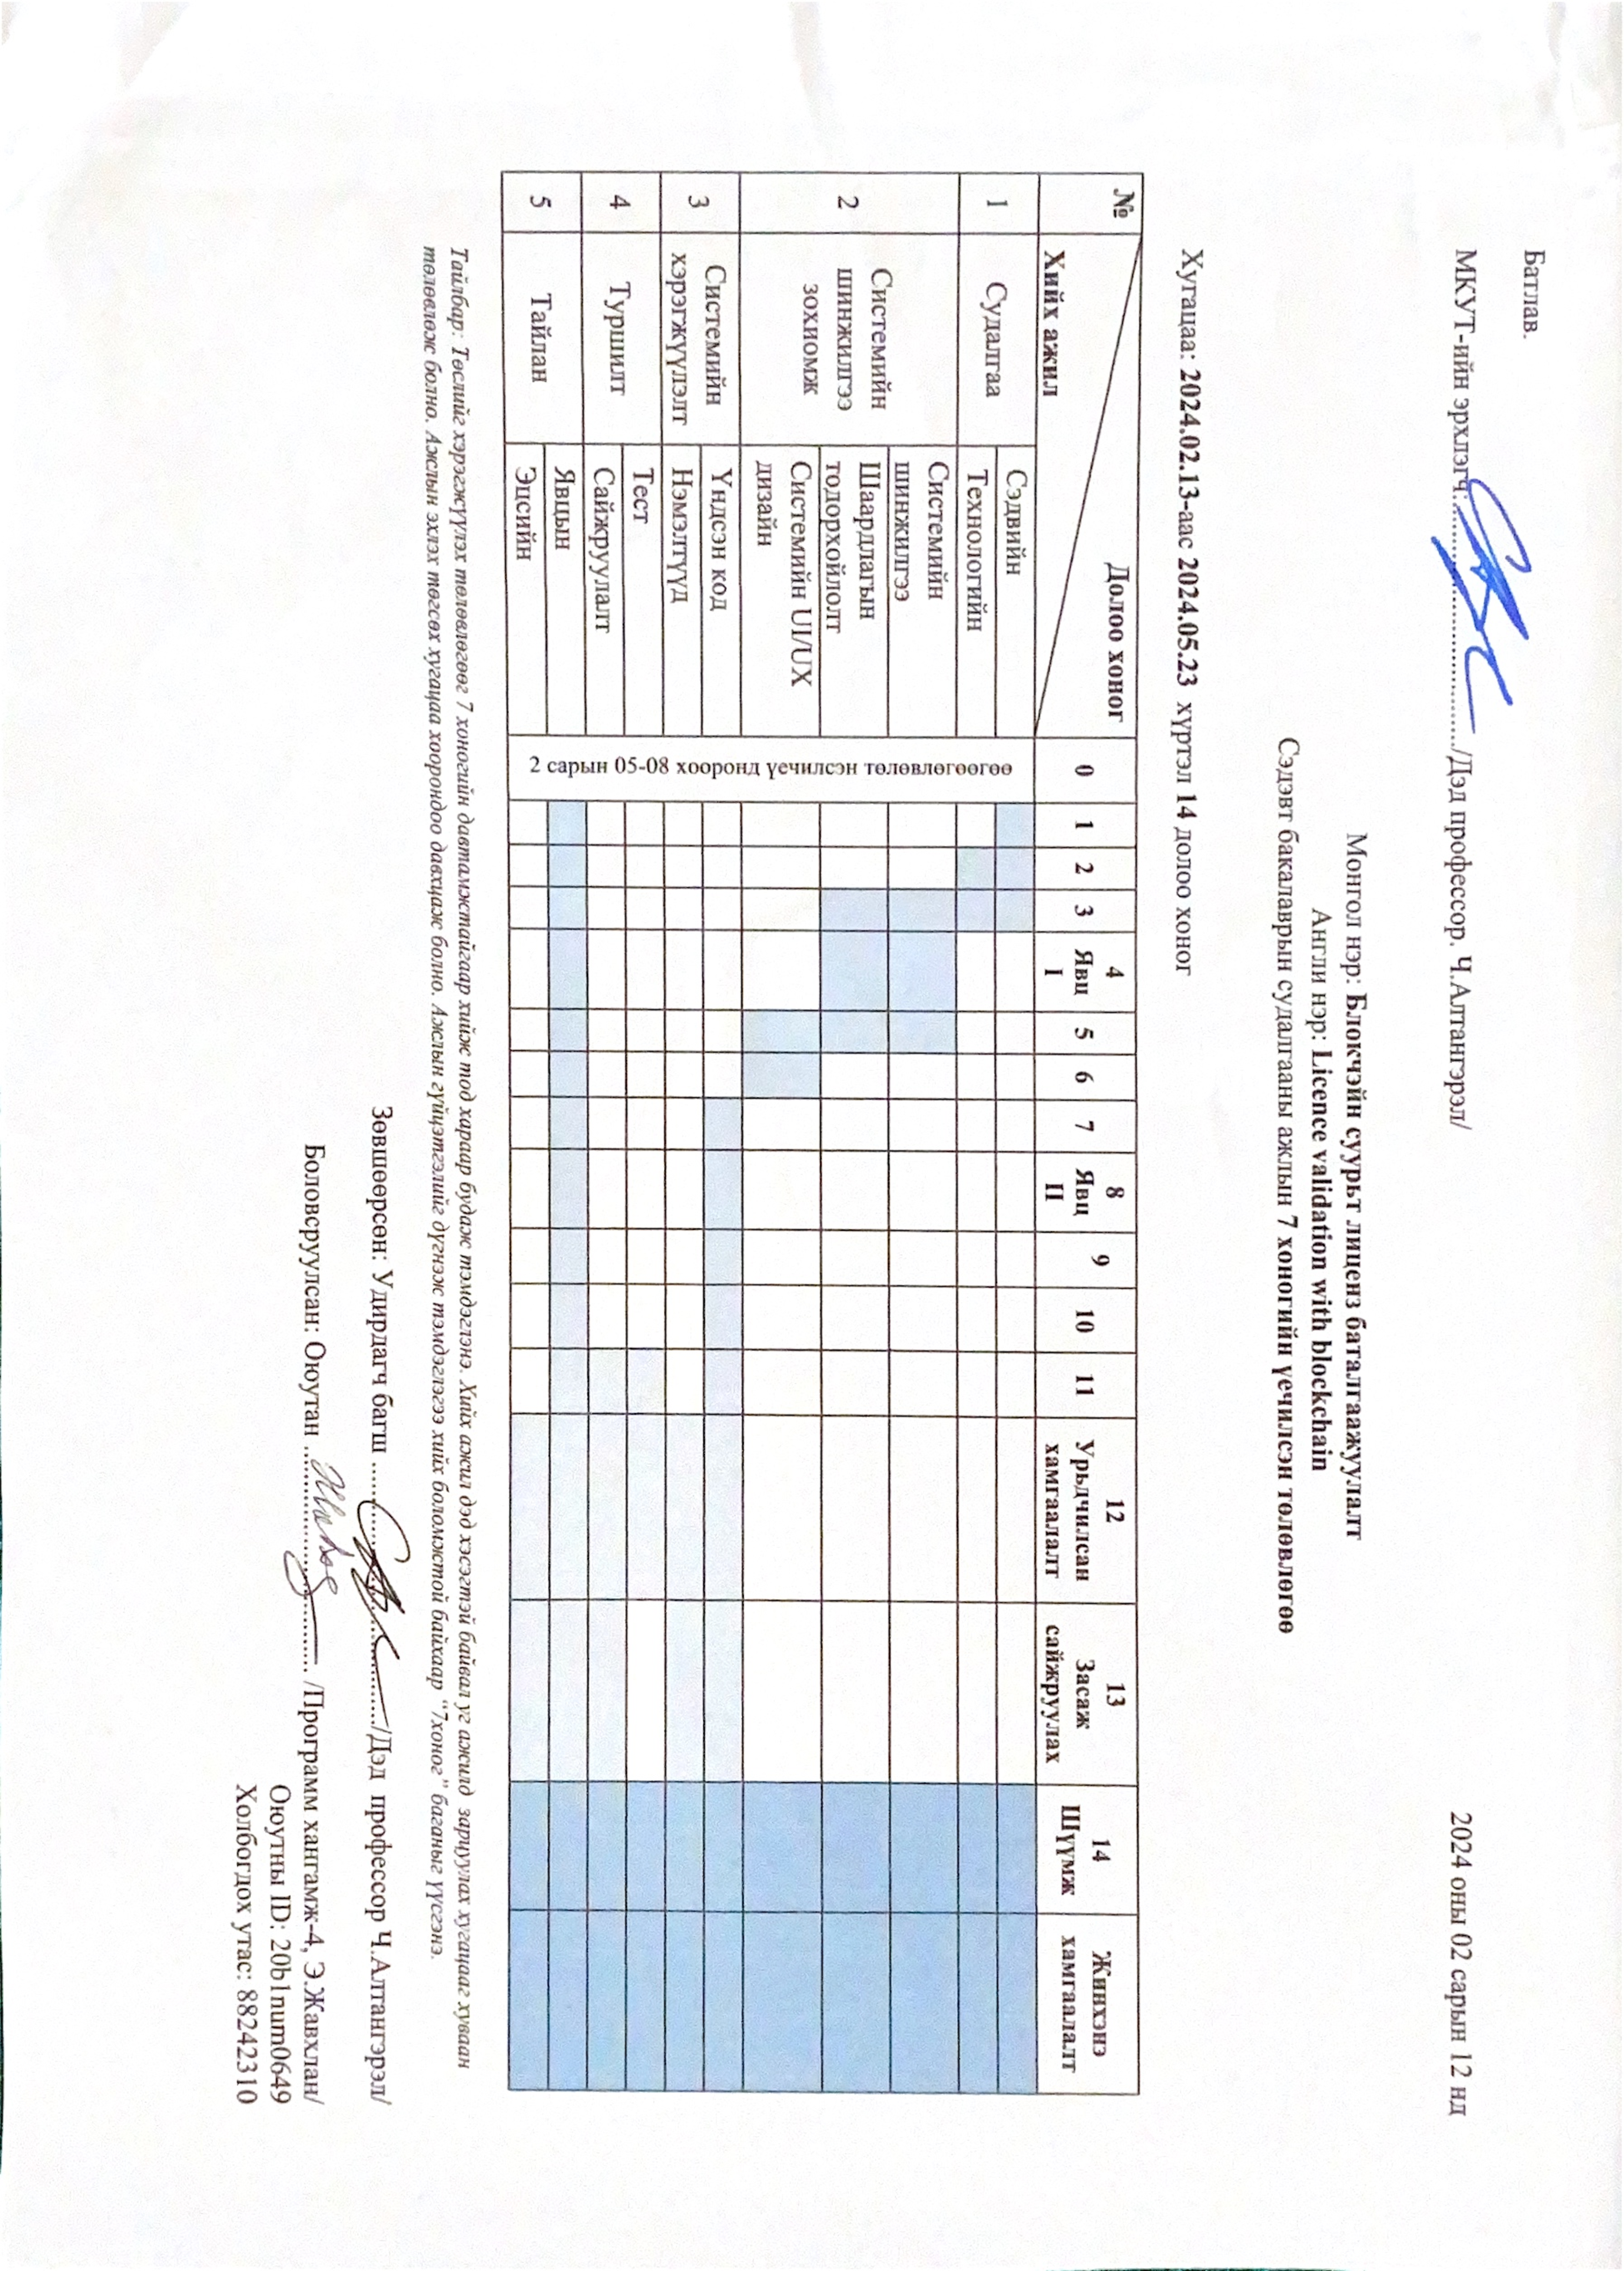
\includepdf[pages=1]{./src/periodic-table.pdf}

\includepdf[pages=1]{./src/todorh.pdf}
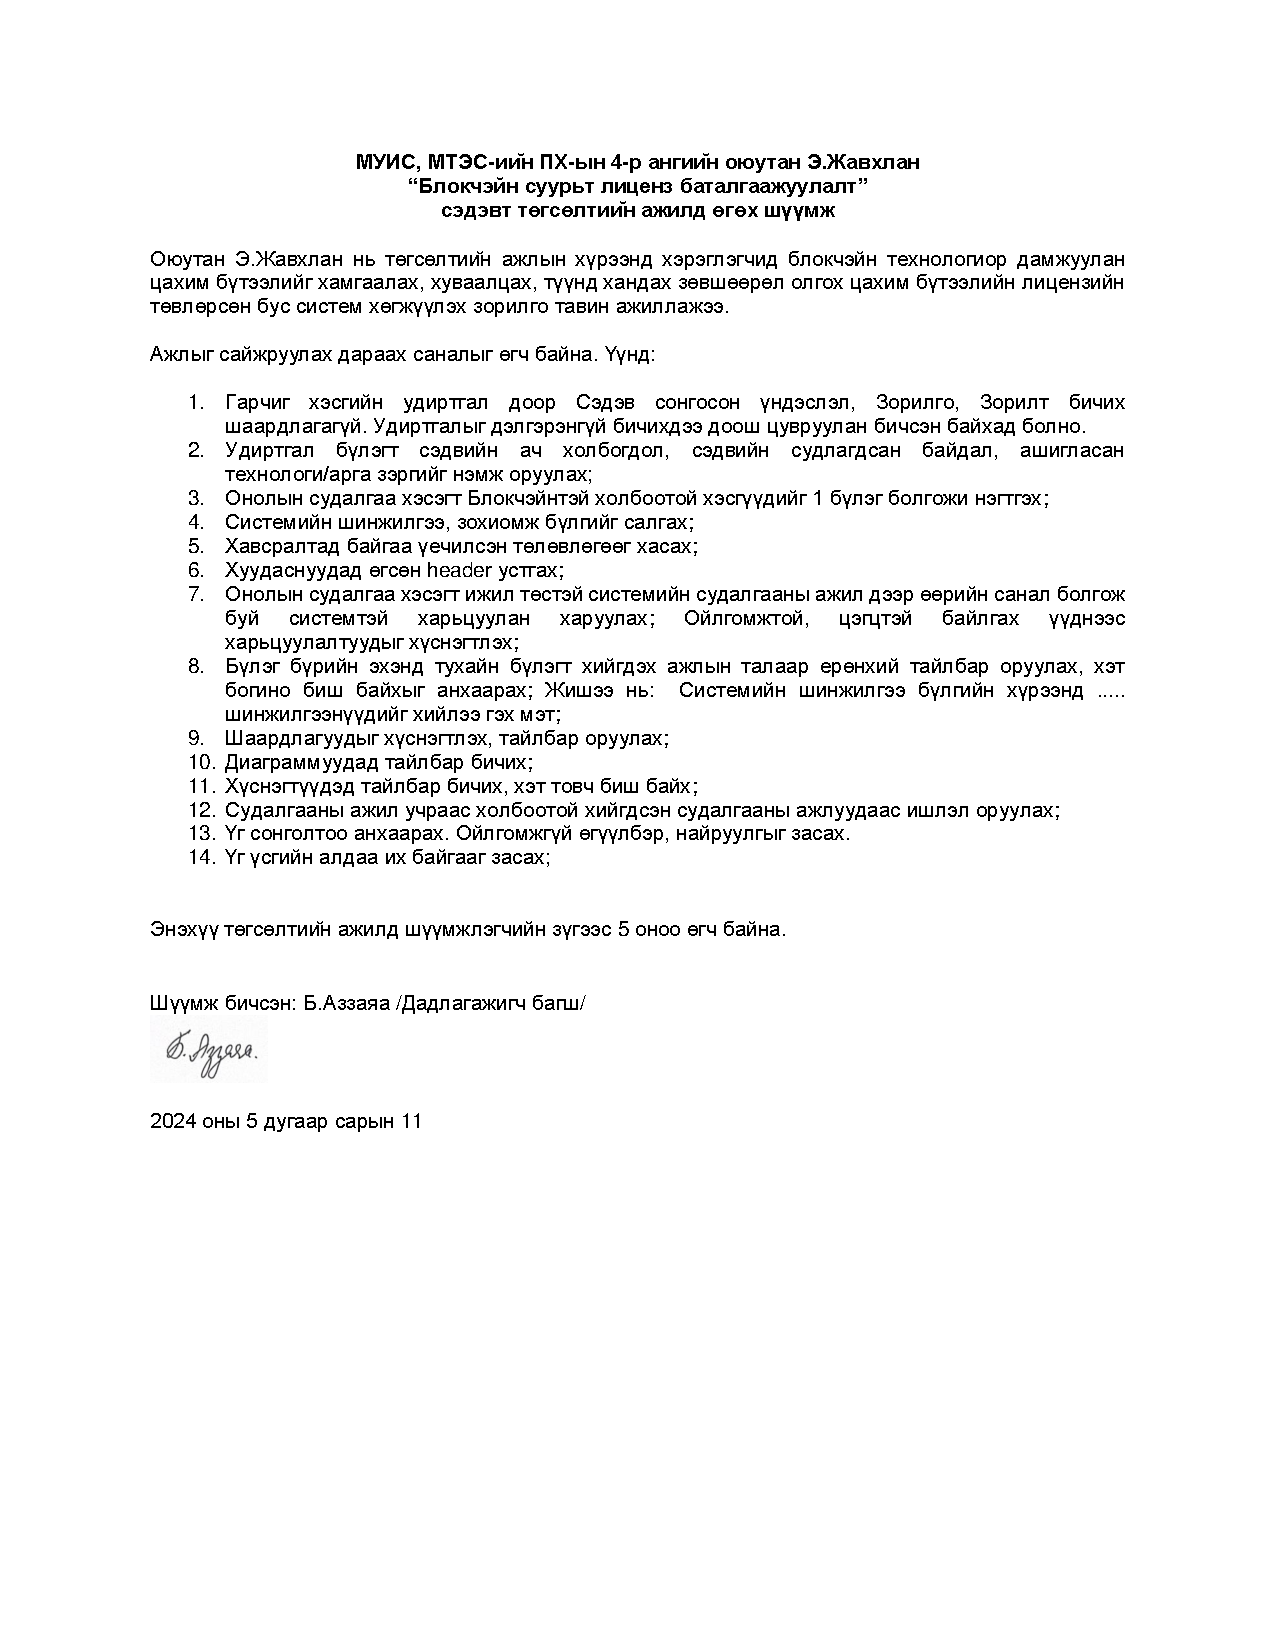
\includepdf[pages=1]{./src/review.pdf}
% Гарчгийг автоматаар оруулна
\setcounter{tocdepth}{1}
\tableofcontents

% Зургийн жагсаалтыг автоматаар оруулна
\listoffigures

% Хүснэгтийн жагсаалтыг автоматаар оруулна
\listoftables

% Кодын жагсаалтыг автоматаар оруулна
\lstlistoflistings

% This puts the word "Page" right justified above everything else.
\newpage
%% \addtocontents{lof}{Зураг~\hfill Хуудас \par}
\newpage
%% \addtocontents{lot}{Хүснэгт~\hfill Хуудас \par}

\renewcommand{\cftlabel}{Зураг}


\doublespace
\pagenumbering{arabic}


% Удиртгалыг оруулж ирэх ба abstract.tex файлд удиртгалаа бичнэ
\begin{abstract}
Миний бие \@author \ үйлдвэрийн дадлагын ажлыг “Зочил технологи” ХХК  компани дээр гүйцэтгэсэн. Энэхүү үйлдвэрийн дадлагын хүрээнд хичээлээс болон бие даан эзэмшсэн мэдлэг, чадвараа ашиглан бодит ажлын орчинд бүтээгдэхүүн хөгжүүлж бодит хэрэглэгчдийн гарт хүргэх процесст суралцан Админ веб удирдлагын систем төслийн front-end хөгжүүлэлтэнд оролцсон.

\textbf{Зорилго:} React, Bootstrap технологиудын талаар судалж бүтээгдэхүүн хөгжүүлэх, компанийн хөгжүүлэлтийн арга барилтай танилцах.

\textbf{Зорилт:} Удирдагчийн зааварчилгааны дагуу алхам алхмаар судалгаа хийж өгсөн шаардлагын хүрээнд хэрэгжүүлэлт хийх. Хурал уулзалтуудад хамрагдаж, бодит бүтээгдэхүүн хөгжүүлэлтийн процесст оролцох. Back-end хөгжүүлэлтийн багтай багаар хамтран ажиллах.

\end{abstract}


%----------------------------------------------------------------------------------------
%   Дипломын үндсэн хэсэг эндээс эхэлнэ
%----------------------------------------------------------------------------------------
\addcontentsline{toc}{part}{БҮЛГҮҮД}
% Шинэ бүлэг
\subfile{src/chapters/chapter1.tex}
\section{Системийн шаардлага}

\subsection{Функционал шаардлагууд}
\begin{itemize}
      \item[] /ФШ 10/ Систем нь цахим бүтээл болон лицензийн талаарх мэдээллийн найдвартай байдлыг хадгалахын тулд блокчэйнтэй харилцах ёстой.
      \item[] /ФШ 20/ Системд хэрэглэгчид крипто хэтэвчээ ашиглан өөрийгөө баталгаажуулах боломжтой байх ёстой (жишээ нь, MetaMask).
      \item[] /ФШ 30/ Системд зөвхөн холбогдсон түрийвчтэй, баталгаажуулсан хэрэглэгчид системийн функцэд хандах эрхтэй байх ёстой.
      \item[] /ФШ 40/ Систем нь хэрэглэгчдэд янз бүрийн төрлийн цахим бүтээлийг (жишээ нь, видео, аудио, PDF, зураг) аюулгүйгээр байршуулах боломжтой байх ёстой.
      \item[] /ФШ 50/ Систем нь цахим бүтээлийг байршуулахдаа бүтээлийн мэдээллийг бүртгэх мөн үнийг тогтоох боломжтой байх ёстой.
      \item[] /ФШ 60/ Систем нь өгөгдлийн нууцлал, аюулгүй байдлыг хангах үүднээс байршуулахаас өмнө файлуудыг шифрлэн IPFS (InterPlanetary File System) дээр найдвартай хадгалах ёстой.
      \item[] /ФШ 70/ Систем нь шифрлэгдсэн файлуудыг зохих зөвшөөрөлтэй эрх бүхий хэрэглэгчдэд зориулан тайлах ёстой.
      \item[] /ФШ 80/ Системд хэрэглэгчдэд цахим бүтээлийн үнэд тохирсон шаардлагатай төлбөрийг төлж эзэмшигчдээс тухайн цахим бүтээлд хандах лиценз буюу хандах зөвшөөрөл авах хүсэлт илгээх боломжтой байх ёстой.
      \item[] /ФШ 90/  Системд цахим бүтээл эзэмшигчид лицензийн хүсэлтийг зөвшөөрөх эсвэл татгалзах боломжтой байх ёстой. Зөвшөөрөгдсөн үед худалдан авагчид бүтээлийн лицензийг өгөх мөн зохих төлбөрийг эзэмшигчид шилжүүлэх ёстой.
      \item[] /ФШ 100/  Системд цахим бүтээл эзэмшигчид мөн хэрэглэгчдийн лицензийн хүсэлтээс татгалзах сонголттой байх ёстой. Ийм тохиолдолд төлбөрийг хэрэглэгчдэд буцааж өгөх ёстой.
      \item[] /ФШ 110/  Систем нь цахим бүтээл эзэмших, түүнд лиценз олгох асуудлыг зохицуулахын тулд ухаалаг гэрээг блокчэйн дээр байршуулж, удирдах ёстой.
      \item[] /ФШ 120/  Системд хэрэглэгчид хүссэн үедээ системээс цахим бүтээлийн орлогоо өөрийн крипто хэтэвч рүү татах боломжтой байх ёстой.
      \item[] /ФШ 130/  Систем нь бүтээл байршуулах, удирдах, өмчлөлийг баталгаажуулахын тулд ухаалаг гэрээтэй харилцах ёстой.
      \item[] /ФШ 140/  Хэрэглэгчид cистем дээр байршуулсан цахим бүтээлийн дэлгэрэнгүй мэдээллийг үзэх боломжтой байх ёстой.
      \item[] /ФШ 150/  Цахим бүтээлийн лиценз авахад лицензэд өвөрмөц дугаар олгож, блокчэйн дээр хадгалах ёстой.
      \item[] /ФШ 160/  Систем нь хэрэглэгчид лиценз авсны дараа лицензийн дугаар, файлын мэдээлэл зэрэг лицензийнхээ дэлгэрэнгүй мэдээллийг агуулсан цахим гэрчилгээ олгох ёстой.
\end{itemize}

\subsection{Функционал бус шаардлагууд}
\begin{itemize}
   \item[] /ФБШ 10/ Блокчэйн технологи нь өгөгдлийн бүрэн бүтэн байдлыг хангаж, лицензийн мэдээллийг зөвшөөрөлгүй өөрчлөхөөс сэргийлнэ.
   \item[] /ФБШ 20/ Систем нь гүйцэтгэлийн бууралтгүйгээр олон тооны хэрэглэгчид болон лицензүүдийг зохицуулах чадвартай байх ёстой.
   \item[] /ФБШ 30/ Ухаалаг гэрээ нь модульчлагдсан байх ёстой бөгөөд шинэчлэгдэхэд хялбар байх ёстой.
   \item[] /ФБШ 40/ Систем нь хүлээн зөвшөөрөгдсөн тодорхой хугацааны дотор баталгаажуулах хүсэлтийг хурдан боловсруулах чадвартай байх ёстой.
   \item[] /ФБШ 50/ Систем нь янз бүрийн техникийн чадвартай хэрэглэгчдэд үүнийг үр дүнтэй ашиглах боломжийг олгодог хэрэглэгчдэд ээлтэй интерфейстэй байх ёстой.
   \item[] /ФБШ 50/ Систем нь янз бүрийн үйлдлийн систем, хөтөч, төхөөрөмжтэй нийцтэй байх ёстой.
   \item[] /ФБШ 60/ Систем нь лиценз олгох, дижитал гүйлгээ, блокчэйн технологитой холбоотой аливаа зохицуулалтын шаардлагад нийцэж байх ёстой.
   \item[] /ФБШ 70/ Энэ систем нь гамшгийн үед өгөгдөл алдагдахгүй байхын тулд найдвартай нөөцлөх, сэргээх механизмтай байх ёстой.
\end{itemize}

\newpage
\section{Системийн ажлын явцын диаграмм}
Цахим бүтээлийн ажлын явцыг дараах байдлаар тодорхойлов. Системийн оролцогч талуудыг цахим бүтээлийн лиценз буюу хандах зөвшөөрөл авах гэж буй хэрэглэгч. Нөгөө талаас цахим бүтээл оруулах, түүнд лиценз буюу хандах зөвшөөрөл олгож буй бүтээл эзэмшигч гэж тодорхойлсон.
\begin{figure}[h!]
	\centering
	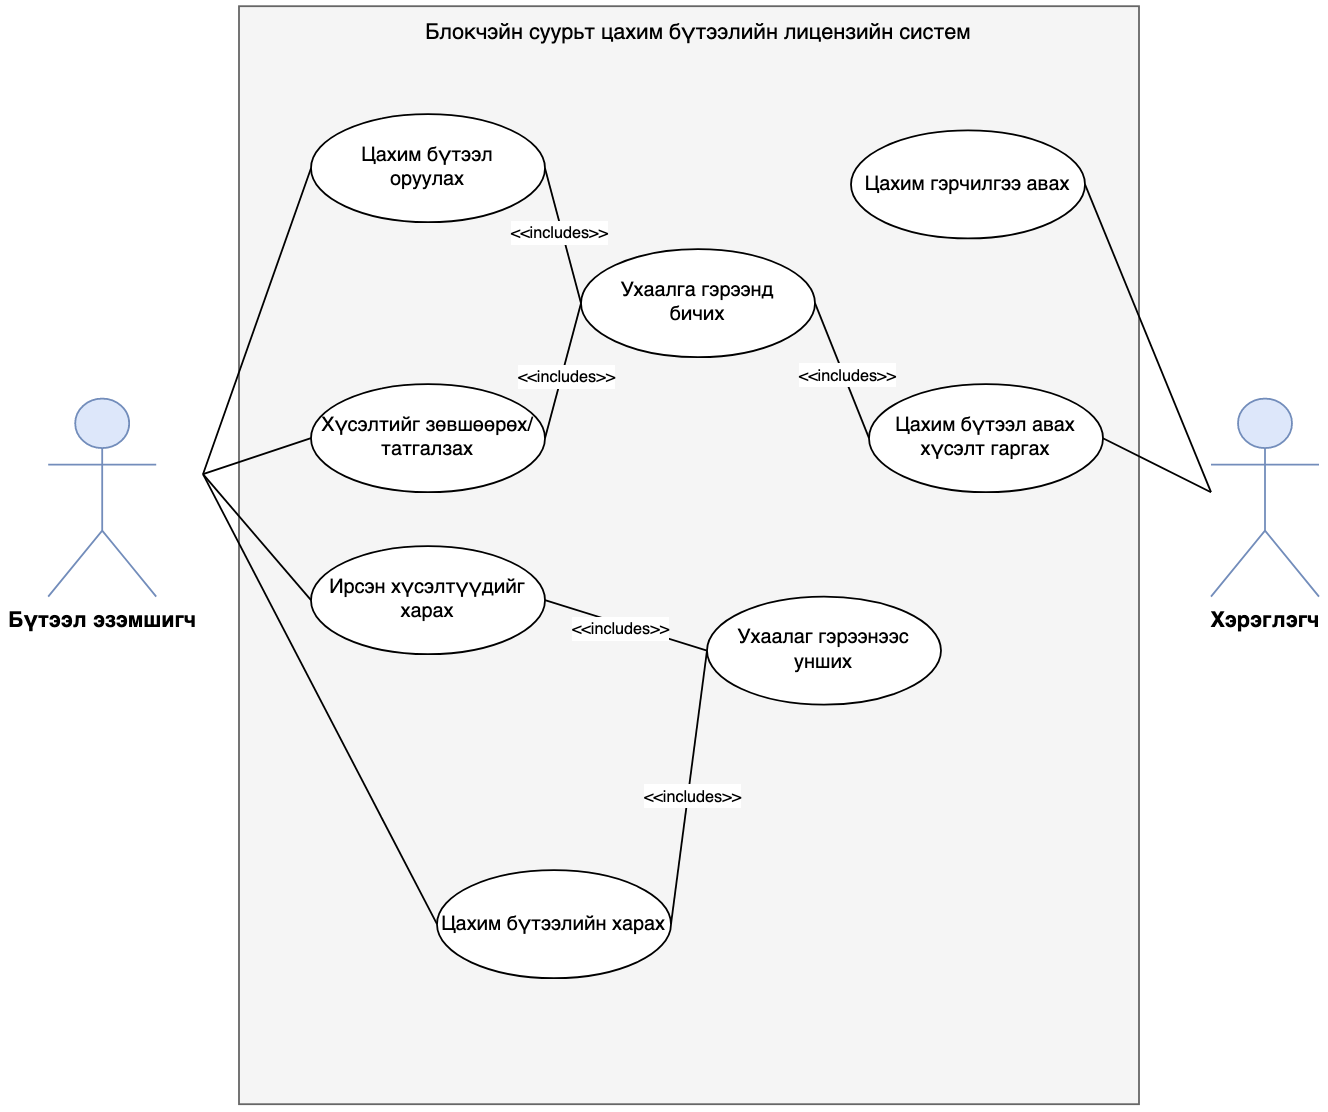
\includegraphics[scale=0.36]{src/images/usecase.png}
	\caption{Use-case диаграмм}
\end{figure}

\pagebreak
\section{Дарааллын диаграмм}
\subsection{Хэрэглэгч цахим бүтээл оруулах дарааллын диаграмм}
\begin{figure}[h!]
	\centering
	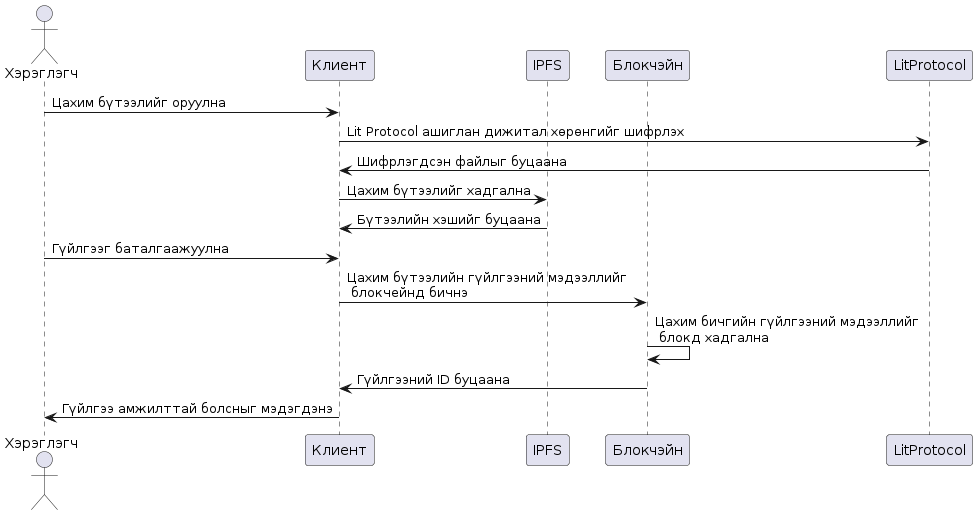
\includegraphics[scale=0.55, angle=90]{src/images/sequence.png}
	\caption{Хэрэглэгч цахим бүтээл оруулах дарааллын диаграмм}
\end{figure}
\subsection{Хэрэглэгч цахим бүтээлд хандах эрх хүсэх дарааллын диаграмм}
\begin{figure}[h!]
	\centering
	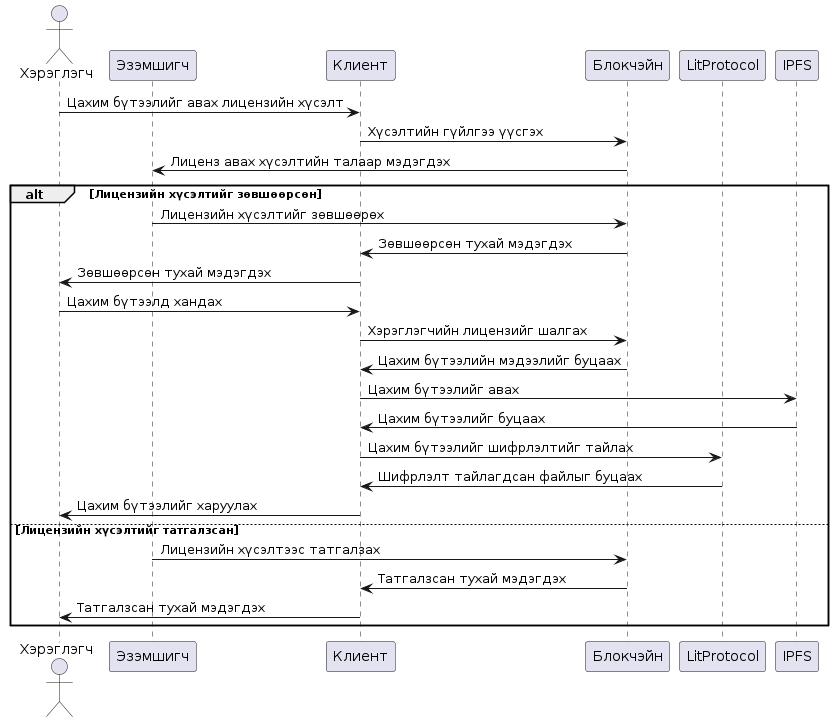
\includegraphics[scale=0.6, angle=90]{src/images/sequence-2.png}
	\caption{Хэрэглэгч цахим бүтээлийг хүсэх дарааллын диаграмм}
\end{figure}

\newpage
\section{Архитектур}
Энэхүү төслийн фронтэнд хэсэг нь NextJS-н ашигласан тул сервер талын рендер хийж байгаа ба хэрэглэгчийн оруулсан цахим бүтээл болон лицензийн мэдээллийг этереум блокчэйн сүлжээнд байршсан ухаалаг гэрээнд бичих болон унших үйлдлийг хийх юм. Мөн хэрэглэгчийн оруулсан цахим бүтээлийн файлыг IPFS сүлжээнд шифрлэн байршуулж, шифрлэлтийн түлхүүрийг Lit сүлжээнд хадгална. Шифрлэлтийн түлхүүрийг хандалтын хяналтын нөхцөлд тодорхойлсны дагуу ухаалаг гэрээгээр зөвшөөрөлтэй эсэхийг шалган авч файлын шифрлэлтийг тайлна.

\begin{figure}[h!]
	\centering
	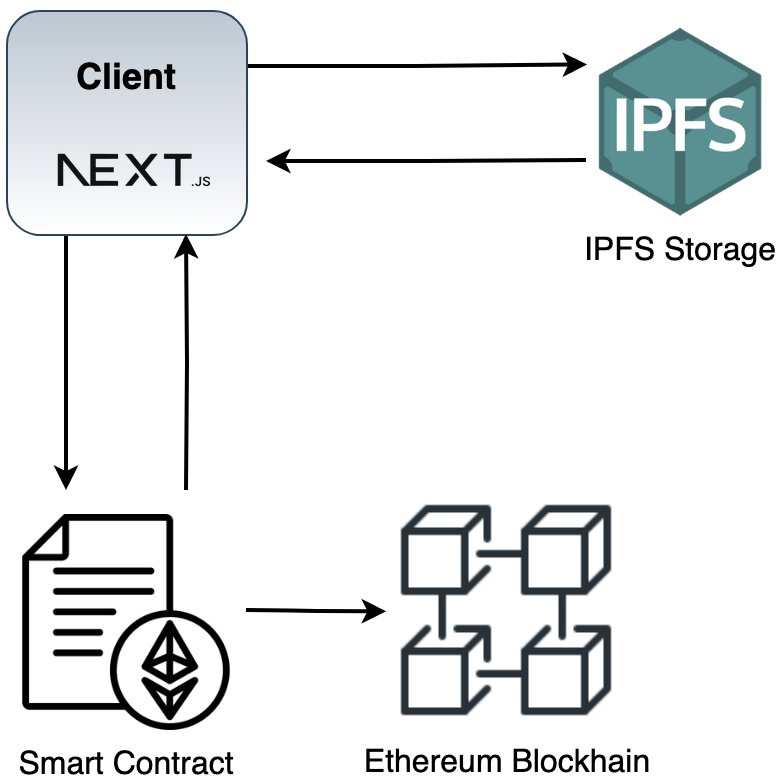
\includegraphics[scale=0.26]{src/images/architecture.png}
	\caption{Системийн ерөнхий архитектур}
\end{figure}

\section{Сонгосон технологи}
\subsection{React \& Next.js}
\subsubsection{Declarative}
React нь хэрэглэгчийн интерактив интерфейс бүтээхийг хялбарчилдаг. Aппликейшны state бүрд зориулсан энгийн бүтэц зохион байгуулахаас гадна, React нь өгөгдөл өөрчлөгдөхөд яг зөв компонентоо өөрчлөн рендер хийдэг. Declarative бүтэц нь кодыг тань debug хийхэд хялбар болгохоос гадна, ажиллагаа нь илүү тодорхой болдог.

\subsubsection{Компонент-д тулгуурласан}
Бие даан state-ээ удирддаг маш энгийн компонент бичиж, эдгээрийг хольж найруулан нарийн бүтэцтэй хэрэглэгчийн интерфейс бүтээх боломжтой. Компонентийн логик нь тэмплэйтээр бус JavaScript-ээр бичигддэг учраас өгөгдлийг апп хооронд хялбар дамжуулж, DOM-оос state-ээ тусад нь байлгаж чадна.

\subsubsection{Next.js}
Netflix, TikTok, Hulu, Twitch, Nike гэсэн орчин үеийн аваргууд ашигладаг энэхүү орчин үеийн фрэймворк нь React технологи дээр үндэслэгдсэн бөгөөд Frontend, Backend хоёр талд хоёуланд нь ажилладаг веб аппуудыг хийх чадвартайгаараа бусдаасаа давуу юм. Next.js-ийн үндсэн дизайн нь клиент болон сервер талын аль алиных давуу талыг ашиглаж чаддаг, ямар нэг дутагдалгүй веб сайтыг яаж хамгийн хурдан хялбар бүтээх вэ гэдгийг бодож тусгасан байдаг. Next.js нь сервер талд react компонентуудыг рендерлэн энгийн html, css, json файл болгон хувиргах замаар ажилладаг бөгөөд 2020 оноос олон нийтэд танигдсан JAMStack технологи болон статик сайт, автоматаар статик хуудас үүсгэх, CDN deployment, сервергүй функц, тэг тохиргоо, файлын системийн рүүтинг (PHP-ээс санаа авсан), SWR (stale while revalidate), сервер талд рендерлэх зэрэг асар олон орчин үеийн шинэхэн технологиудыг бүгдийг хийж чаддаг анхны бүрэн веб фрэймворк гэж хэлж болно.

\subsection{Ethereum блокчэйн}
Төвлөрсөн бус, блокчэйн дээр суурилсан программуудыг хангамжийн платформ анх Ethereum-ийг 2013 онд программист Vitalik Buterin бичсэн бөгөөд 2015 онд олон нийтэд анх танилцуулагдсан юм. Ethereum нь бусад койныг бодвол зөвхөн арилжааны бус тус платформыг ашиглан smart contract буюу ухаалаг гэрээ үүсгэх боломжтой. Энэ нь энгийнээр хөгжүүлэгчдэд төвлөрсөн бус хэрэглээний программуудыг бүтээх, ажиллуулах боломжийг олгодог.

\subsection{Hardhat}
Hardhat нь ухаалаг гэрээг хөгжүүлэх орчин юм. Энэ нь Ethereum ухаалаг гэрээг бичих, туршихаас эхлээд байршуулах, дибаг хийх хүртэлх бүх амьдралын мөчлөгийг хөнгөвчлөх зорилготой юм. Hardhat нь Ethereum Virtual Machine (EVM) дээр бүтээгдсэн бөгөөд Ethereum, Polygon, Avalanche болон бусад EVM-тэй нийцтэй блокчэйнүүдийг дэмждэг.

\subsection{Wagmi}
Wagmi нь блокчэйнтэй ажиллахад шаардлагатай бүх зүйлийг агуулсан React Hook-ийн цуглуулга юм. Wagmi нь крифто түрийвч холбох, мэдээллийг авах, ухаалаг гэрээтэй харилцах гэх мэт үйлдлүүдийг хөнгөвчлөх боломжийг олгодог.

\subsection{IPFS \& Pinata}
IPFS буюу Interplanetary File System нь peer-to-peer сүлжээн дэх файлуудыг хадгалах, хуваалцахад зориулагдсан төвлөрсөн бус протокол юм. Үндсэндээ IPFS нь файлуудыг жижиг хэсгүүдэд хувааж, сүлжээний олон зангилаанд хадгалдаг. Энэ нь файлуудыг нэг байршилд хадгалдаггүй, харин сүлжээгээр тарааж байршуулдаг.
Pinata нь төвлөрсөн бус бичиг баримт хадгалалтын сүлжээ болох Interplanetary File System (IPFS) дээр бүтээгдсэн үйлчилгээ юм. Pinata нь хөгжүүлэгчид болон хэрэглэгчдэд IPFS сүлжээнд өгөгдөл хадгалах, уншихад хялбар болгодог. Энэ нь IPFS дээр хадгалагдсан файлуудыг байршуулах, удирдах, хандахад зориулсан API болон бусад хэрэгслээр хангаснаар IPFS-тэй харилцах үйл явцыг хялбаршуулдаг.

\subsection{Lit Protocol}
Lit Protocol нь өөр өөр талууд эсвэл программуудын хооронд аюулгүй, хувийн харилцаа холбоо, өгөгдөл дамжуулах боломжийг олгодог төвлөрсөн бус сүлжээний протокол юм. Энэ нь одоо байгаа блокчэйн болон төвлөрсөн бус хадгалалтын шийдлүүдийн дээр нууцлал, хандалтын хяналтын давхаргыг хангах зорилготой юм.

Lit Protocol-н хэд хэдэн гол технологи, ойлголтууд:
\begin{itemize}
   \item  End-to-End Шифрлэлт: Протокол нь талуудын хооронд хуваалцсан өгөгдөл нь нууц хэвээр үлдэж, зөвхөн хүссэн хүлээн авагчид хандах боломжтой байхын тулд төгсгөлөөс төгсгөл хүртэл шифрлэлтийг ашигладаг.
   \item  Хандалтын хяналтын нөхцөлүүд: Lit Protocol нь хандалтын хяналтын нөхцөлийн тухай ойлголтыг танилцуулсан бөгөөд энэ нь хэн тодорхой өгөгдөлд хандах эсвэл тодорхой үйлдлийг гүйцэтгэх боломжтой болохыг тодорхойлдог криптограф нотолгоо юм. Эдгээр нөхцөлүүд нь төвлөрсөн бус байдлаар хэрэгжиж, төвлөрсөн эрх мэдлийн хэрэгцээг арилгадаг.
   \item Төвлөрсөн бус таних тэмдэг: Протокол нь аюулгүй харилцаа холбоо, мэдээлэл солилцох үйл ажиллагаанд оролцож буй талуудыг төлөөлөхийн тулд Ethereum хаяг эсвэл блокчэйнд суурилсан бусад таних тэмдэг зэрэг төвлөрсөн бус таних тэмдгийг ашигладаг.
\end{itemize}

Энэхүү судалгааны ажлын хүрээнд хэрэглэгчийн байршуулсан файлуудыг шифрлэх, файлуудад хандах хандалтыг хянахад найдвартай, төвлөрсөн бус шийдлээр хангах зорилгоор Lit Protocol-ийг сонгосон. Lit Protocol-тэй нэгтгэснээр систем нь файлуудыг найдвартай хадгалж, хандалтын хяналтын тодорхой нөхцөөл дээр үндэслэн зөвхөн эрх бүхий этгээдэд хандах боломжтой.

\newpage
\section{Хөгжүүлэлт}

\subsection{Хөгжүүлэлтийн орчныг бэлдэх}
Энэхүү судалгааны ажлын практик хэсэгт би NextJS, Hardhat, Pinata, Wagmi, Tailwind CSS зэргийг ашиглан хөгжүүлэлт хийх билээ. NextJS нь монолитик төсөл хийхэд тохиромжтой ба төслийн ухаалаг гэрээ хөгжүүлэлт, клайнт талуудыг нэг repository-д хадгалж байгаа. Version Control System-ээр Github-г сонгосон юм. Кодын фолдер бүтэц нь дараах байдлаар байна.

\begin{figure}[h]
	\centering
	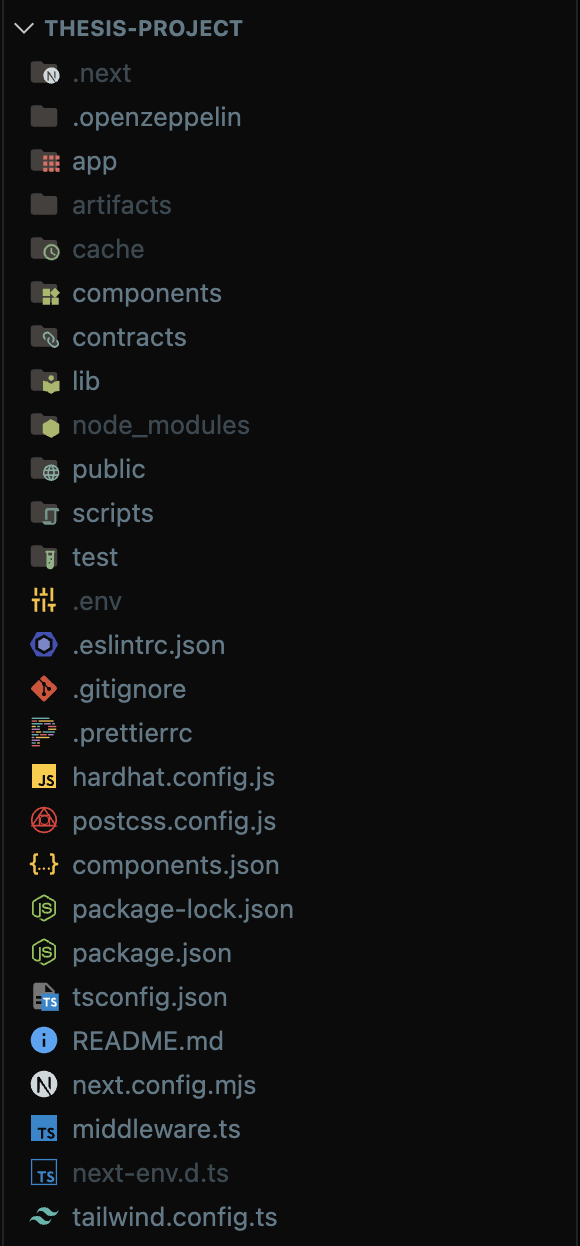
\includegraphics[scale=0.3]{src/images/folder-structure.png}
	\caption{Фолдерийн бүтэц}
\end{figure}

\begin{itemize}
	\item \textbf{components} - React компонентууд
	\item \textbf{lib} - Хэрэглэгчийн талын шаардлагатай код туслах функцууд
	\item \textbf{app} - NextJS дээрх хуудаснууд
	\item \textbf{public} - Статик зураг, файлууд
	\item \textbf{scripts} - Ухаалаг гэрээний хөгжүүлэлтийн холбоотой  javascript файлууд
	\item \textbf{contracts} - Ухаалаг гэрээний файлууд
\end{itemize}

\subsection{Ухаалаг гэрээн хөгжүүлэлт}
Миний төсөл нэг ухаалаг гэрээнээс бүтнэ. Уг ухаалаг гэрээ нь цахим файлууд болон тэдгээртэй холбоотой лицензүүдийг төлөөлдөг Файл ба Лиценз гэсэн хоёр бүтцийг тодорхойлсон.
Файл бүтэц  нь id, эзэмшигчийн хаяг, файлын нэр, тайлбар, ангилал, файлын хэш, үүсгэсэн хугацааны  зэрэг атрибутуудыг агуулна.
Лиценз бүтэц нь лицензийн дугаар, эзэмшигчийн хаяг, файлын нэр, тайлбар, ангилал, файлын хэш, үүсгэсэн хугацааны  зэрэг атрибутуудыг агуулна.
Мөн дараах функцүүдтэй:

\begin{itemize}
	\item \textbf{createFile}: Цахим баримт бичгийн мэдээллийг бичих
	\item \textbf{issueLicense}: Лицензийн мэдээллийг бичих
	\item \textbf{getAllPublicFiles}: Оруулсан бүх цахим баримт бичгийн авах
	\item \textbf{getAllUserFiles}:  Хэрэглэгчийн оруулсан цахим баримт бичгүүдийг авах
	\item \textbf{getAllUserLicenses}: Хэрэглэгчийн эзэмшиж буй лицензүүдийг авах
	\item \textbf{validateLicense}: Лицензийн дугаараар лицензийг шалгах
	\item \textbf{getPublicFileById}: Цахим баримт бичгийг  авах id-гаар нь авах
	\item \textbf{getMarketplaceFiles}: Лиценз авах боломжтой цахим баримт бичгүүдийг авах
	\item \textbf{generateUniqueLicense}: Лицензд өвөрмөц дугаар бий болгох
\end{itemize}

\subsection{Ухаалаг гэрээг блокчэйнд байршуулах}
\lstinputlisting[language=TypeScript,caption=deploy,basicstyle=\linespread{0.8}\ttfamily,frame=single]{src/code/deploy.js}

\subsection{Хэрэглэгч талын хөгжүүлэлт (Front-end)}
Уг код нь хэрэглэгчийн оруулах цахим баримт бичгийн мэдээллийг блокчэйнд бичнэ.
\lstinputlisting[language=TypeScript, caption=Блокчэйнд бичих,basicstyle=\linespread{0.8}\ttfamily,frame=single]{src/code/writeFile.ts}

Энэ функц нь хэрэглэгчийн оруулсан баримт бичгийг IPFS-д байршуулна.
\lstinputlisting[language=TypeScript, caption=Файл IPFS-д  байршуулах,basicstyle=\linespread{0.8}\ttfamily,frame=single]{src/code/uploadIpfs.ts}

Уг код нь хэрэглэгчийн оруулсан цахим баримт бичгүүдийн мэдээллийг блокчэйнээс уншина.
\lstinputlisting[language=TypeScript, caption=Блокчэйнээс унших,basicstyle=\linespread{0.8}\ttfamily,frame=single]{src/code/getUserFiles.ts}


\pagebreak
\subsection{Үр дүн}
Төслийн практик ажлын үр дүнд бүтээгдсэн  системийн интерфейс дараах байдлаар харагдана.
\begin{figure}[h!]
	\centering
	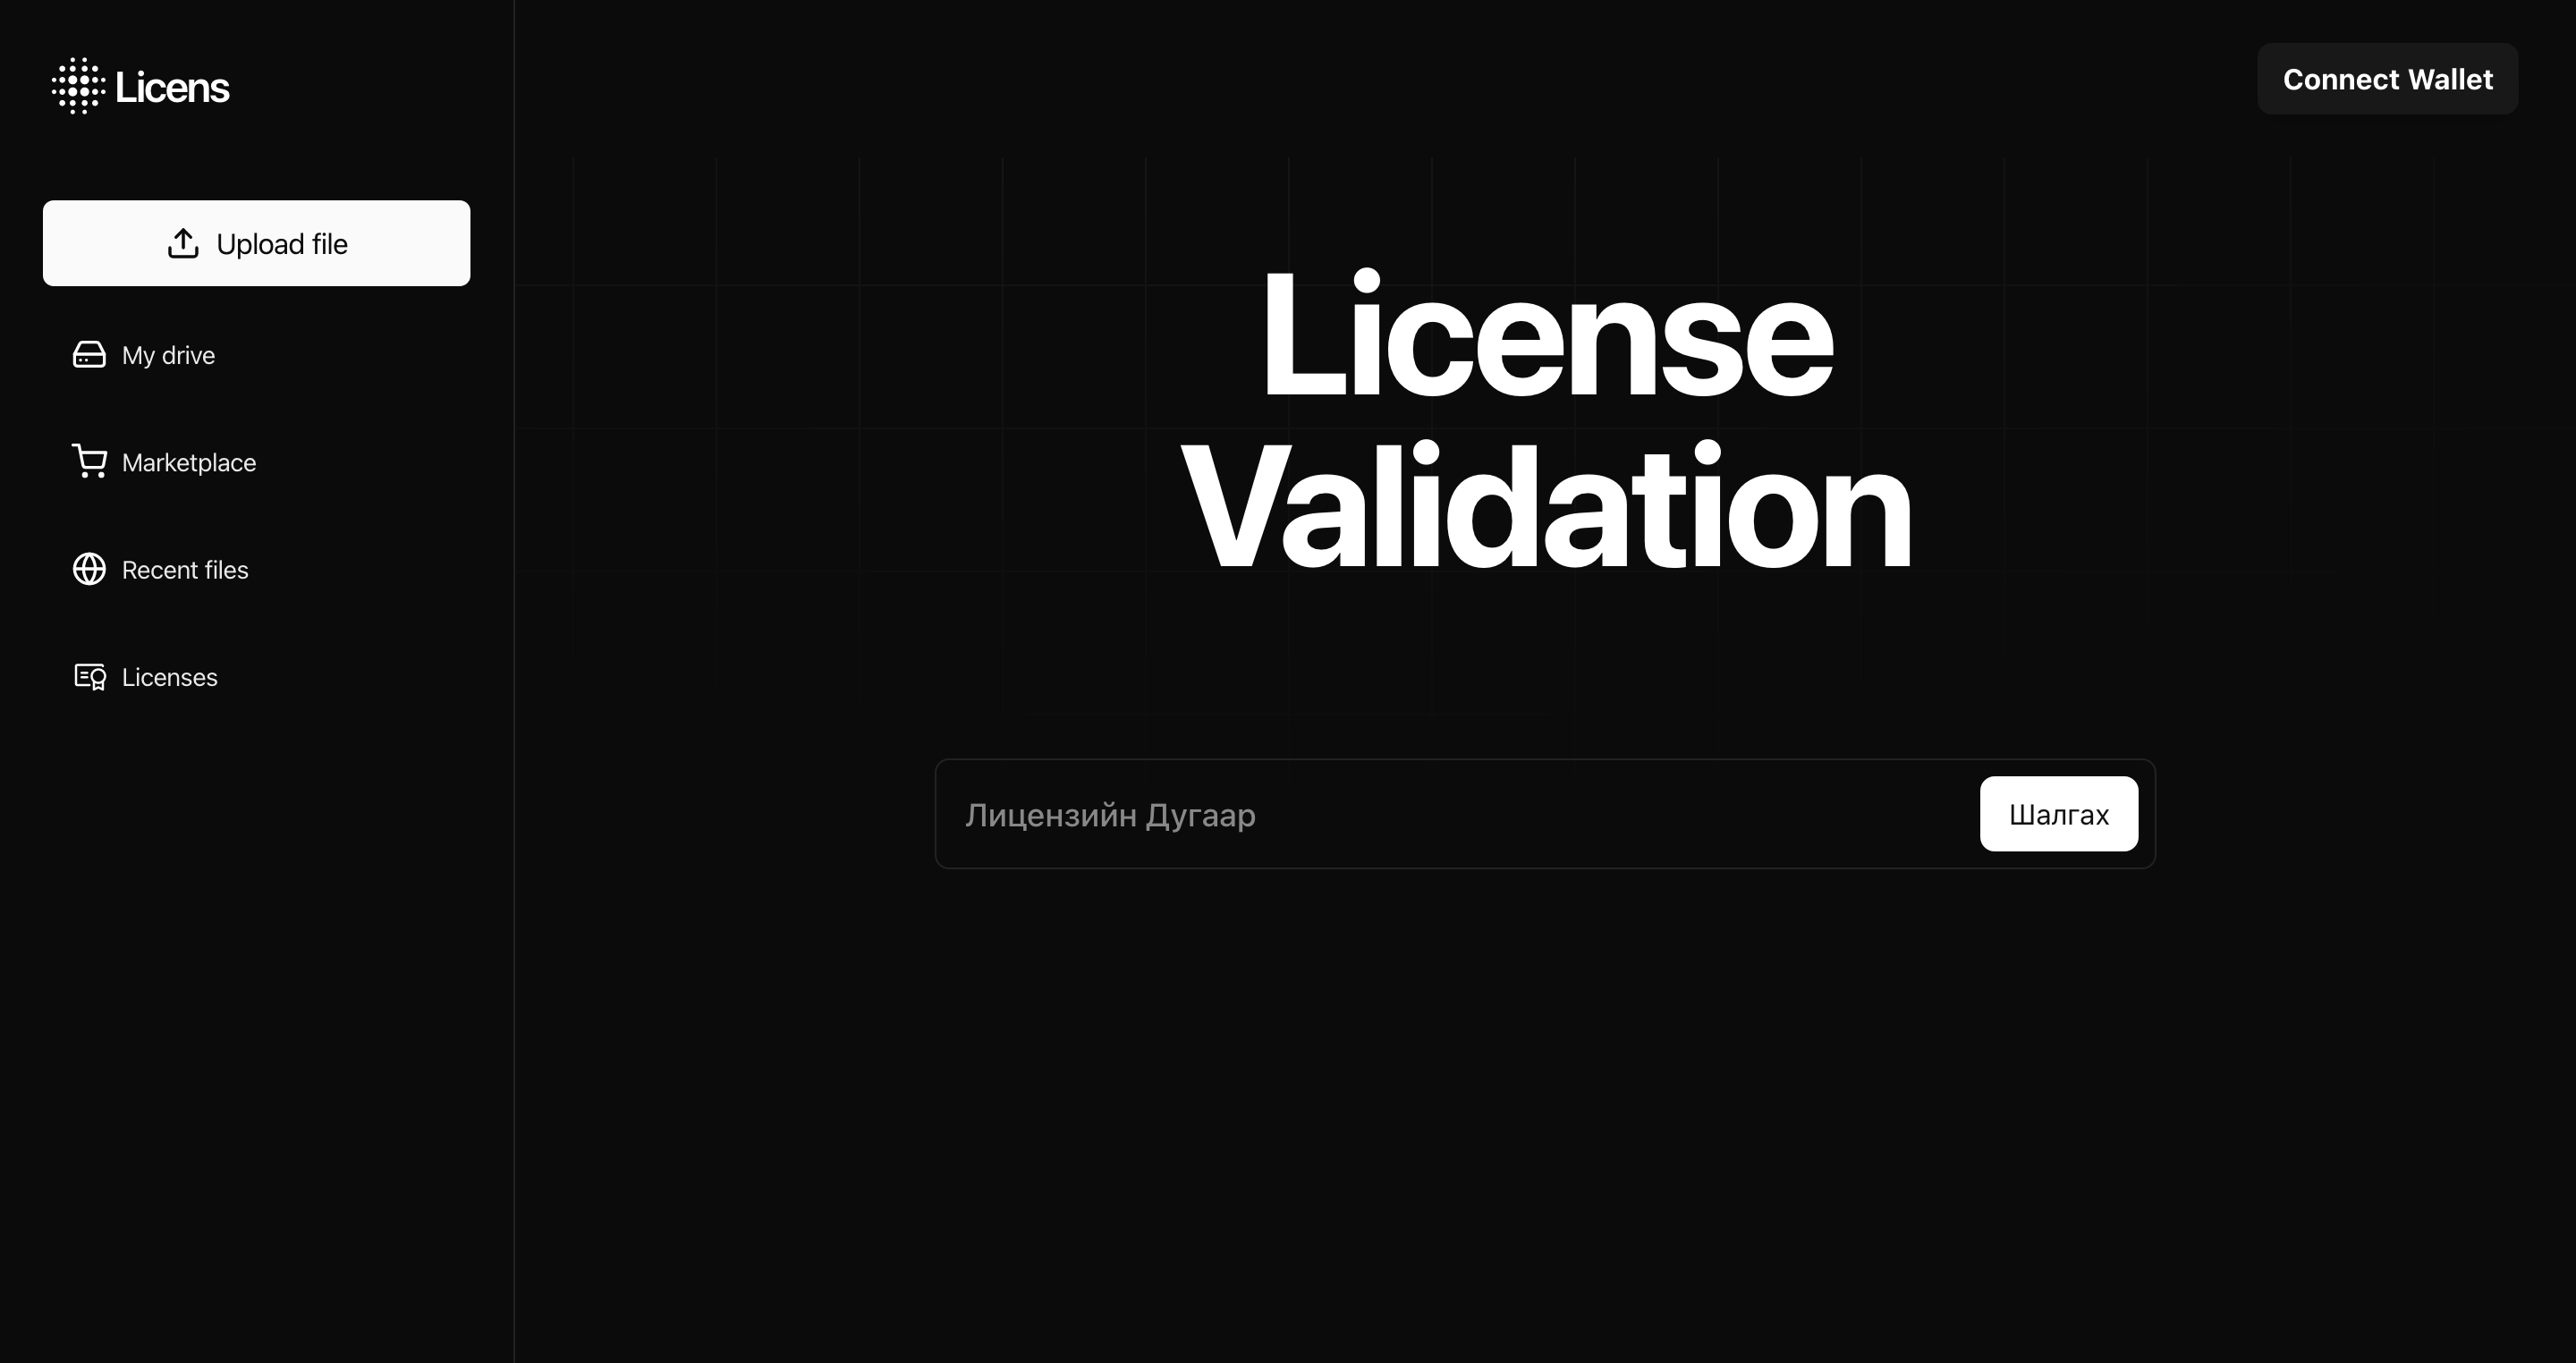
\includegraphics[scale=0.155]{src/images/homepage.png}
	\caption{Нүүр хуудас}
\end{figure}

\begin{figure}[h!]
	\centering
	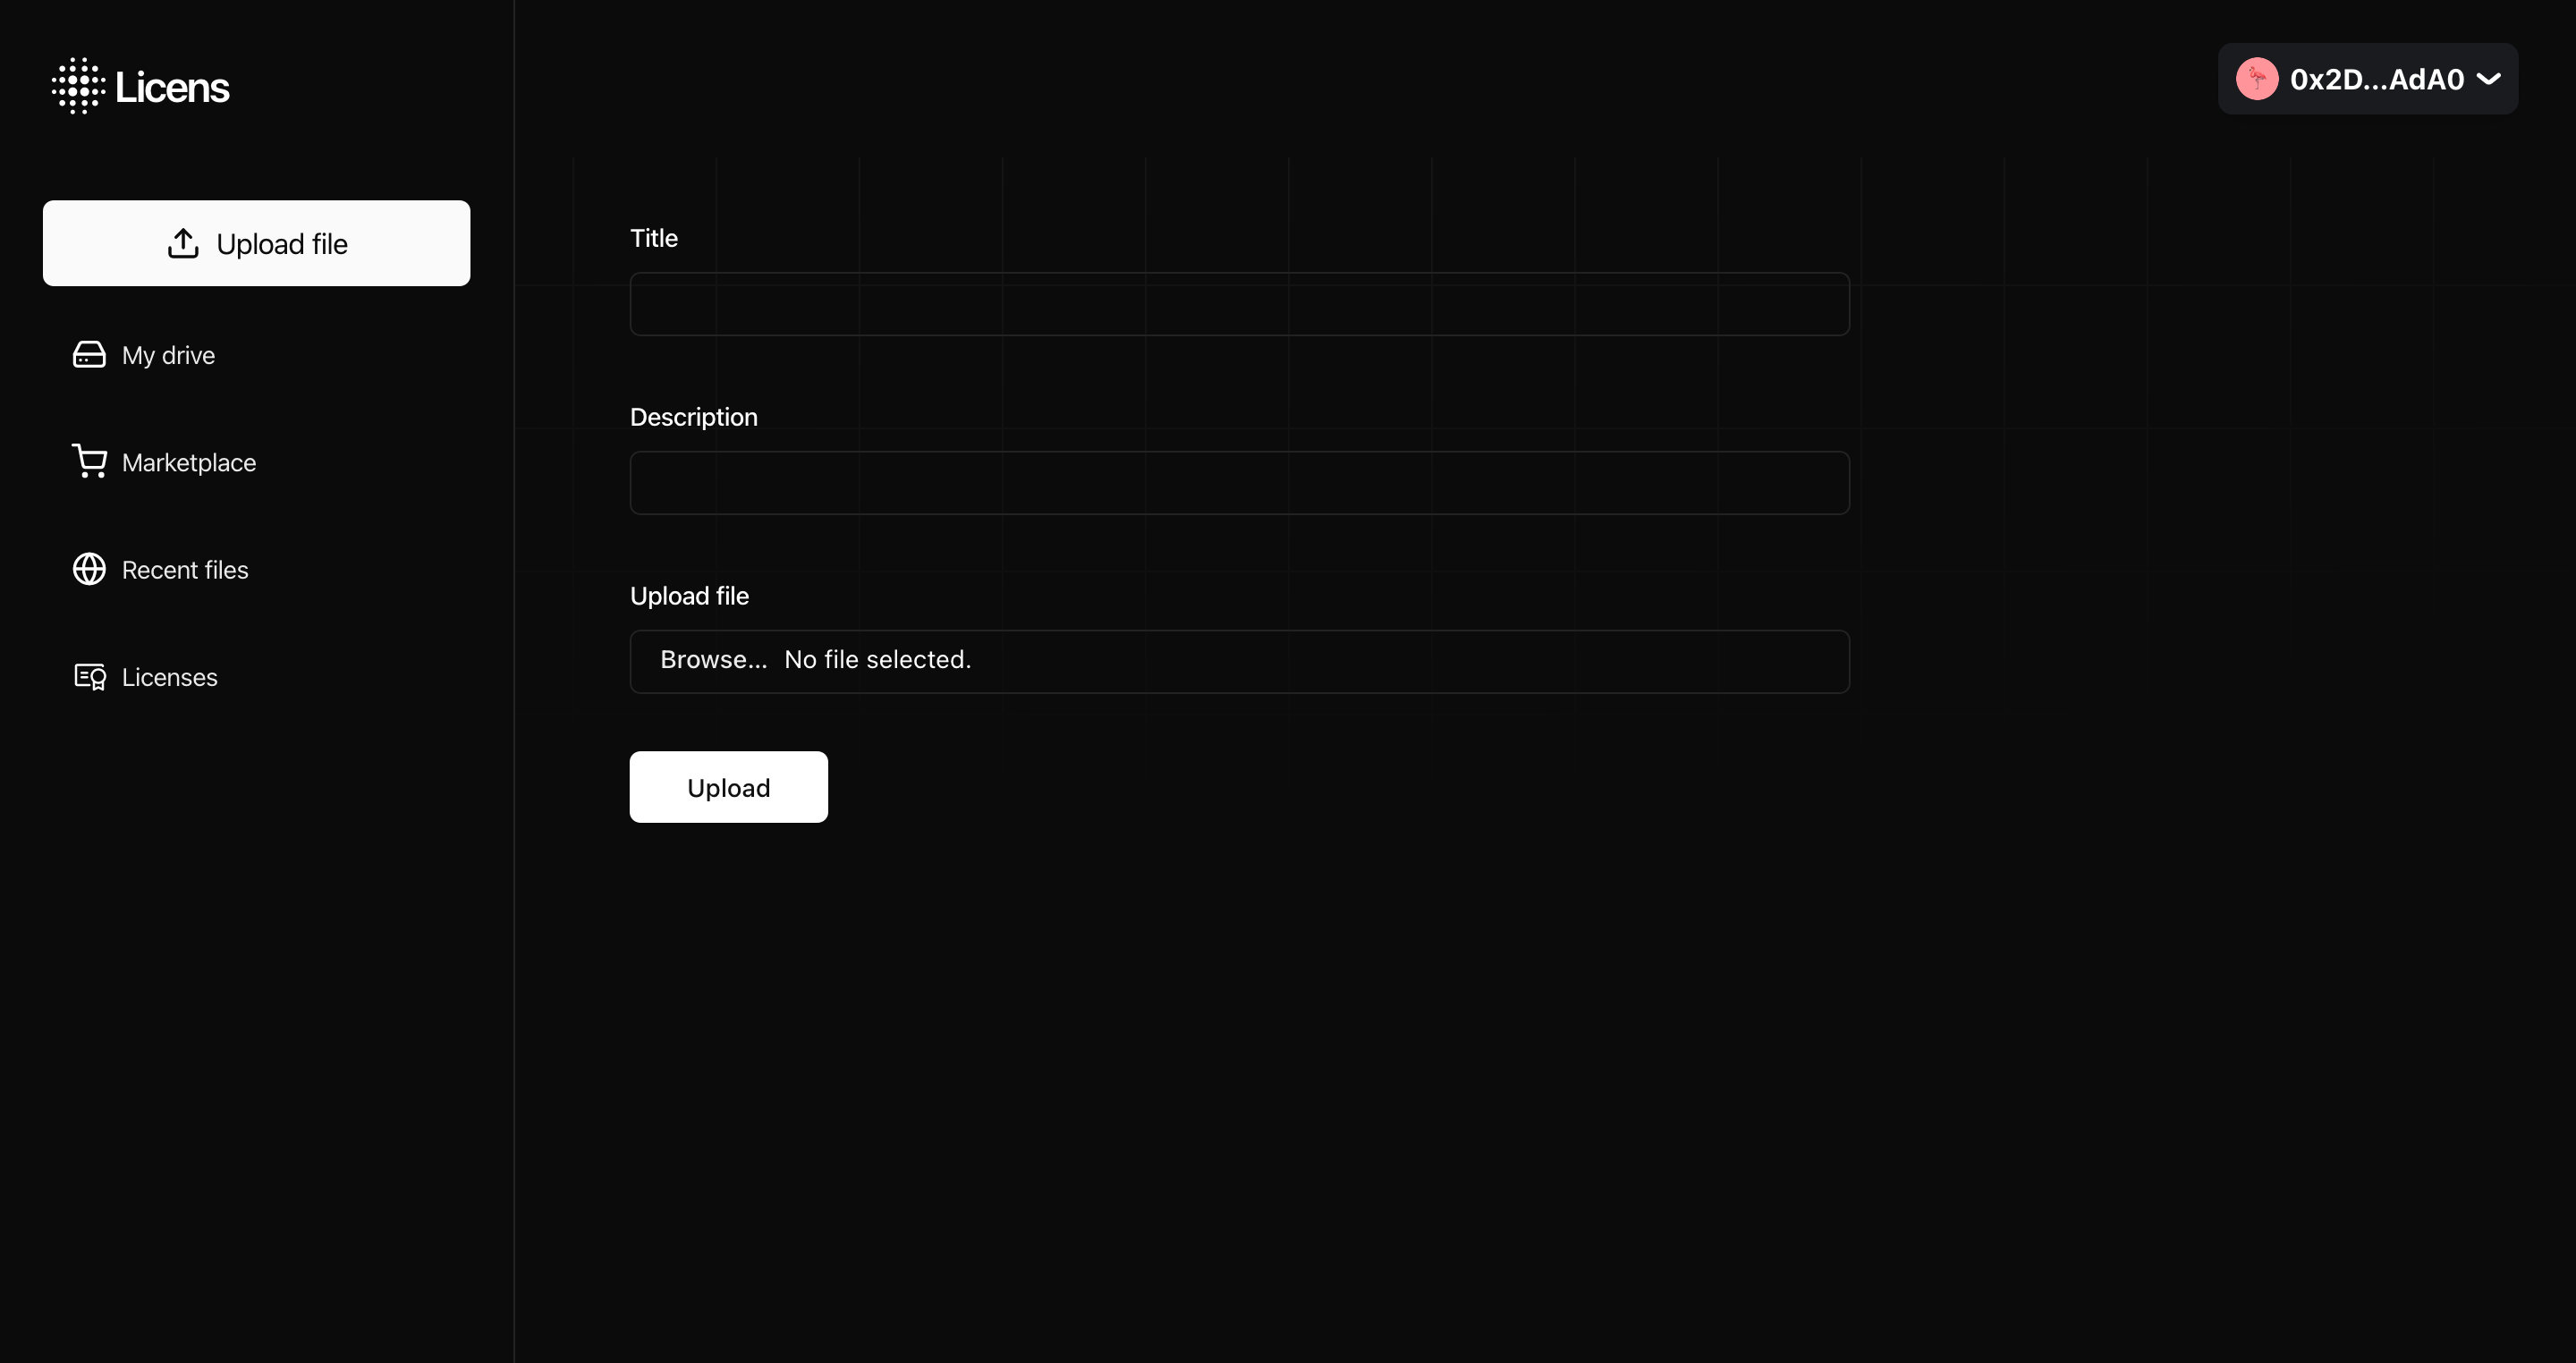
\includegraphics[scale=0.155]{src/images/upload-page.png}
	\caption{Цахим бичиг баримт оруулах}
\end{figure}

\begin{figure}[h!]
	\centering
	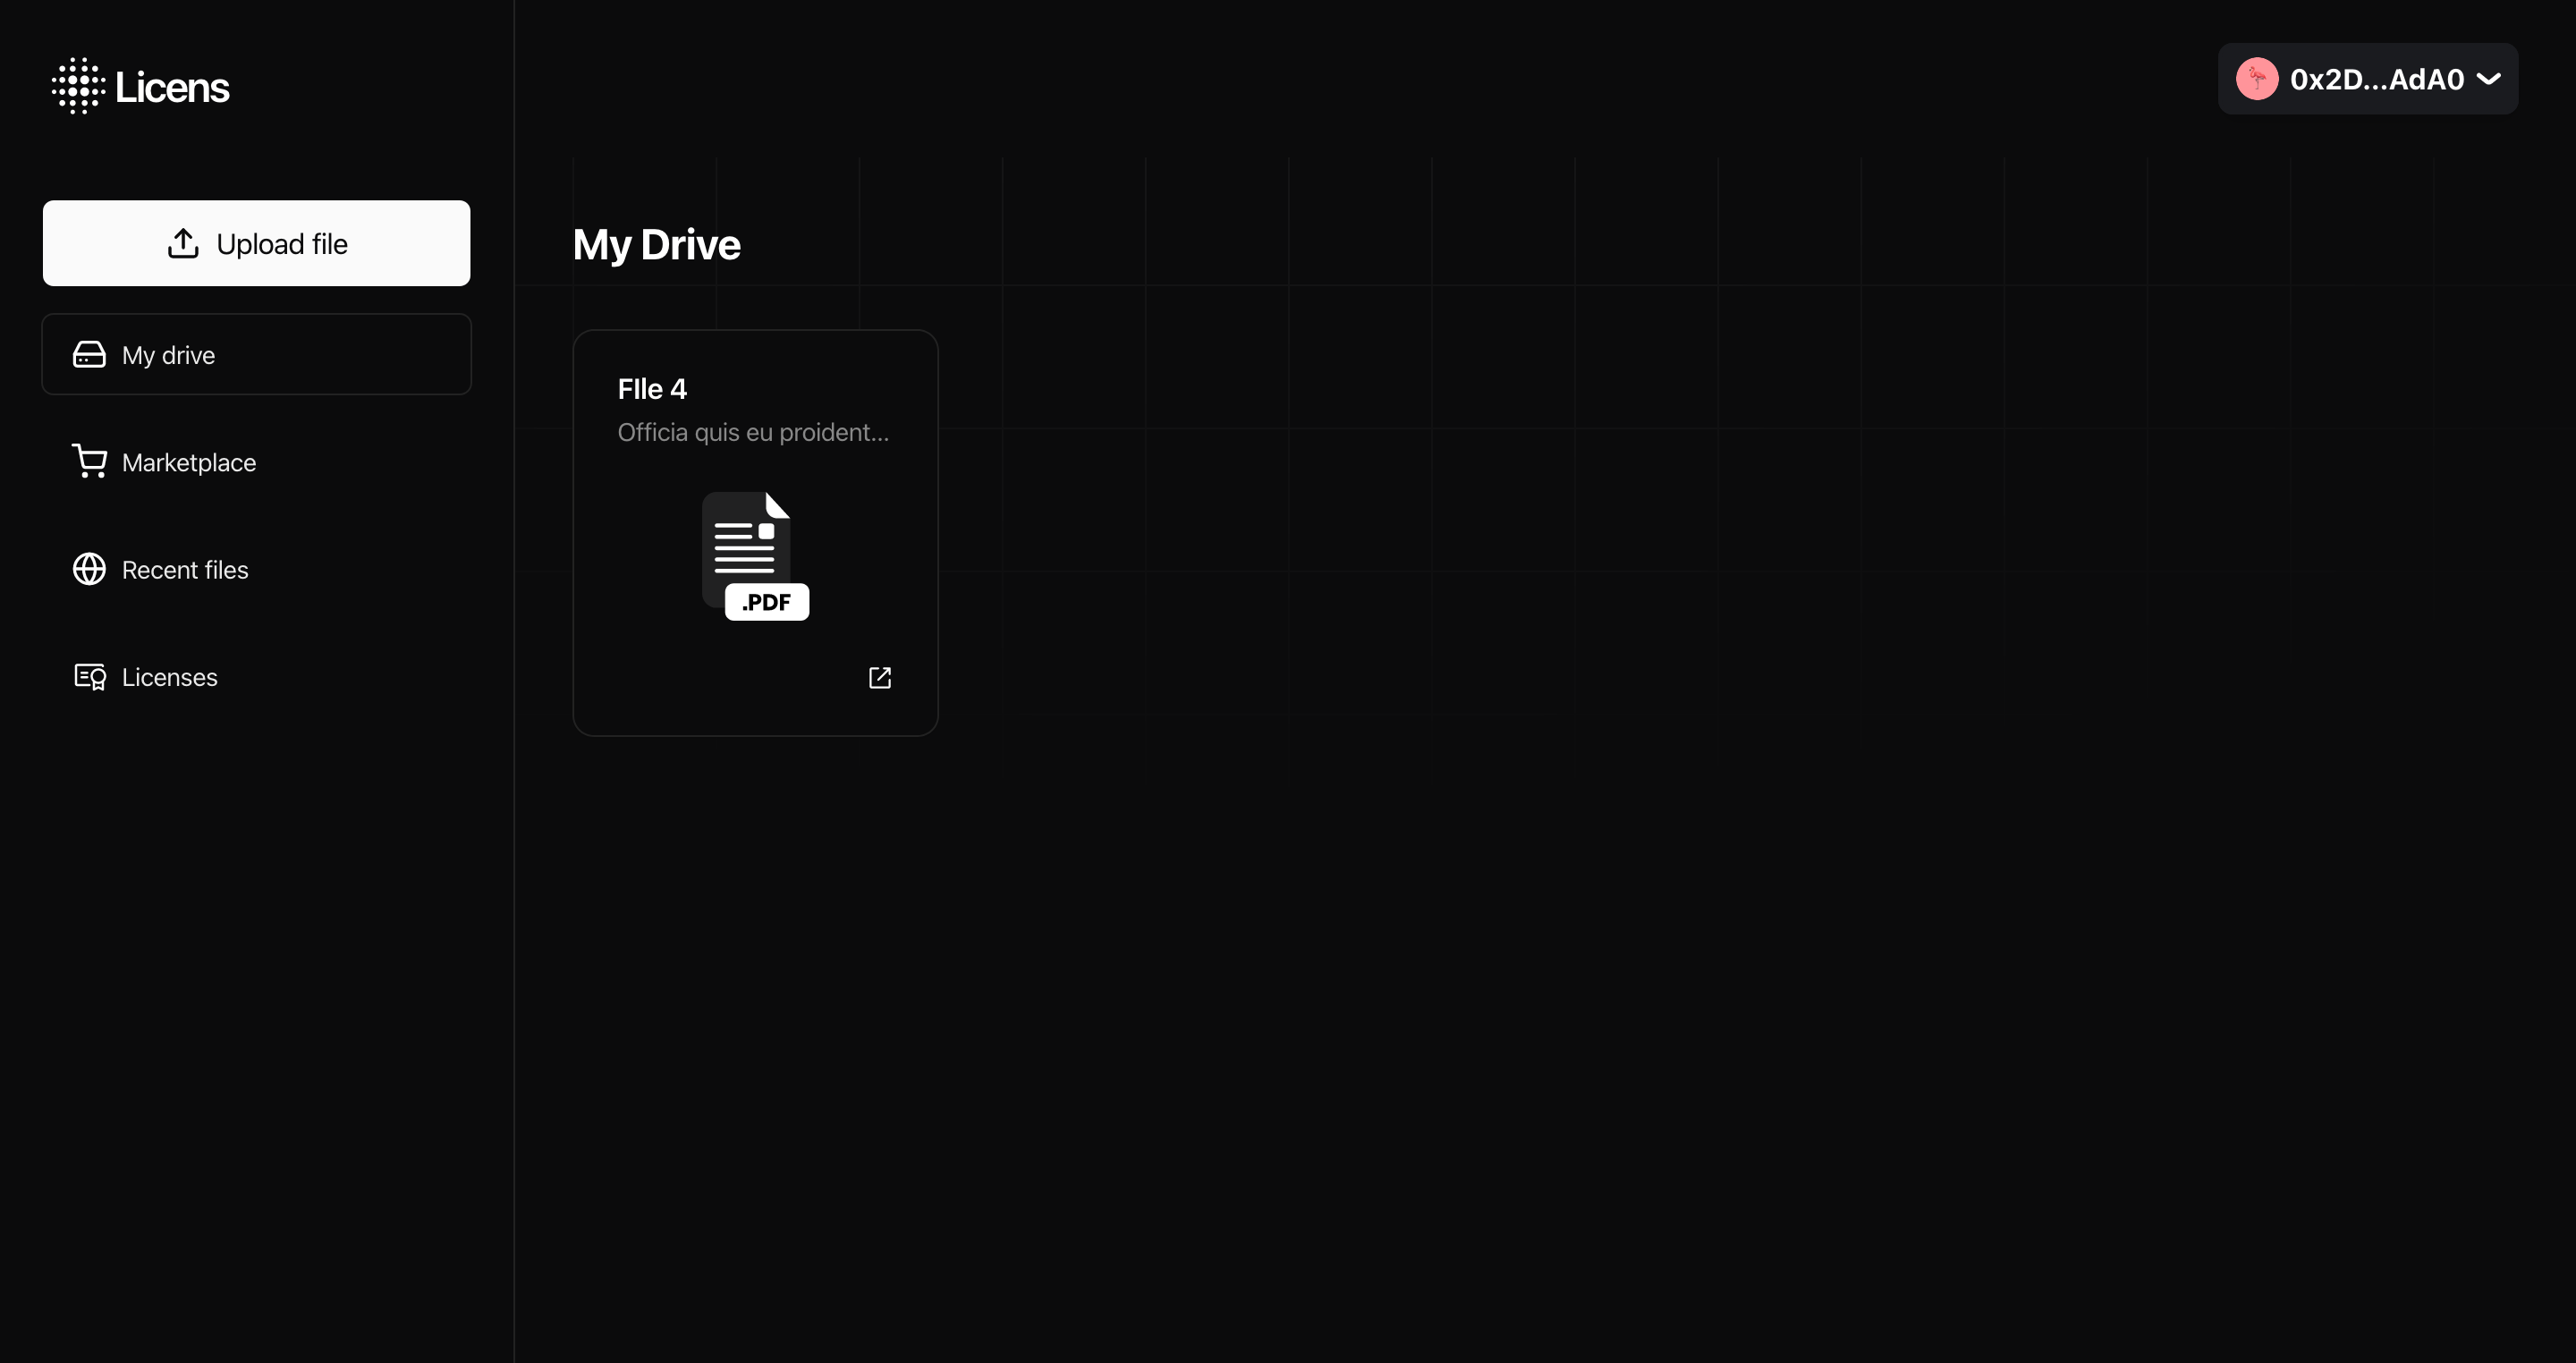
\includegraphics[scale=0.165]{src/images/drive-page.png}
	\caption{}
\end{figure}

\begin{figure}[h!]
	\centering
	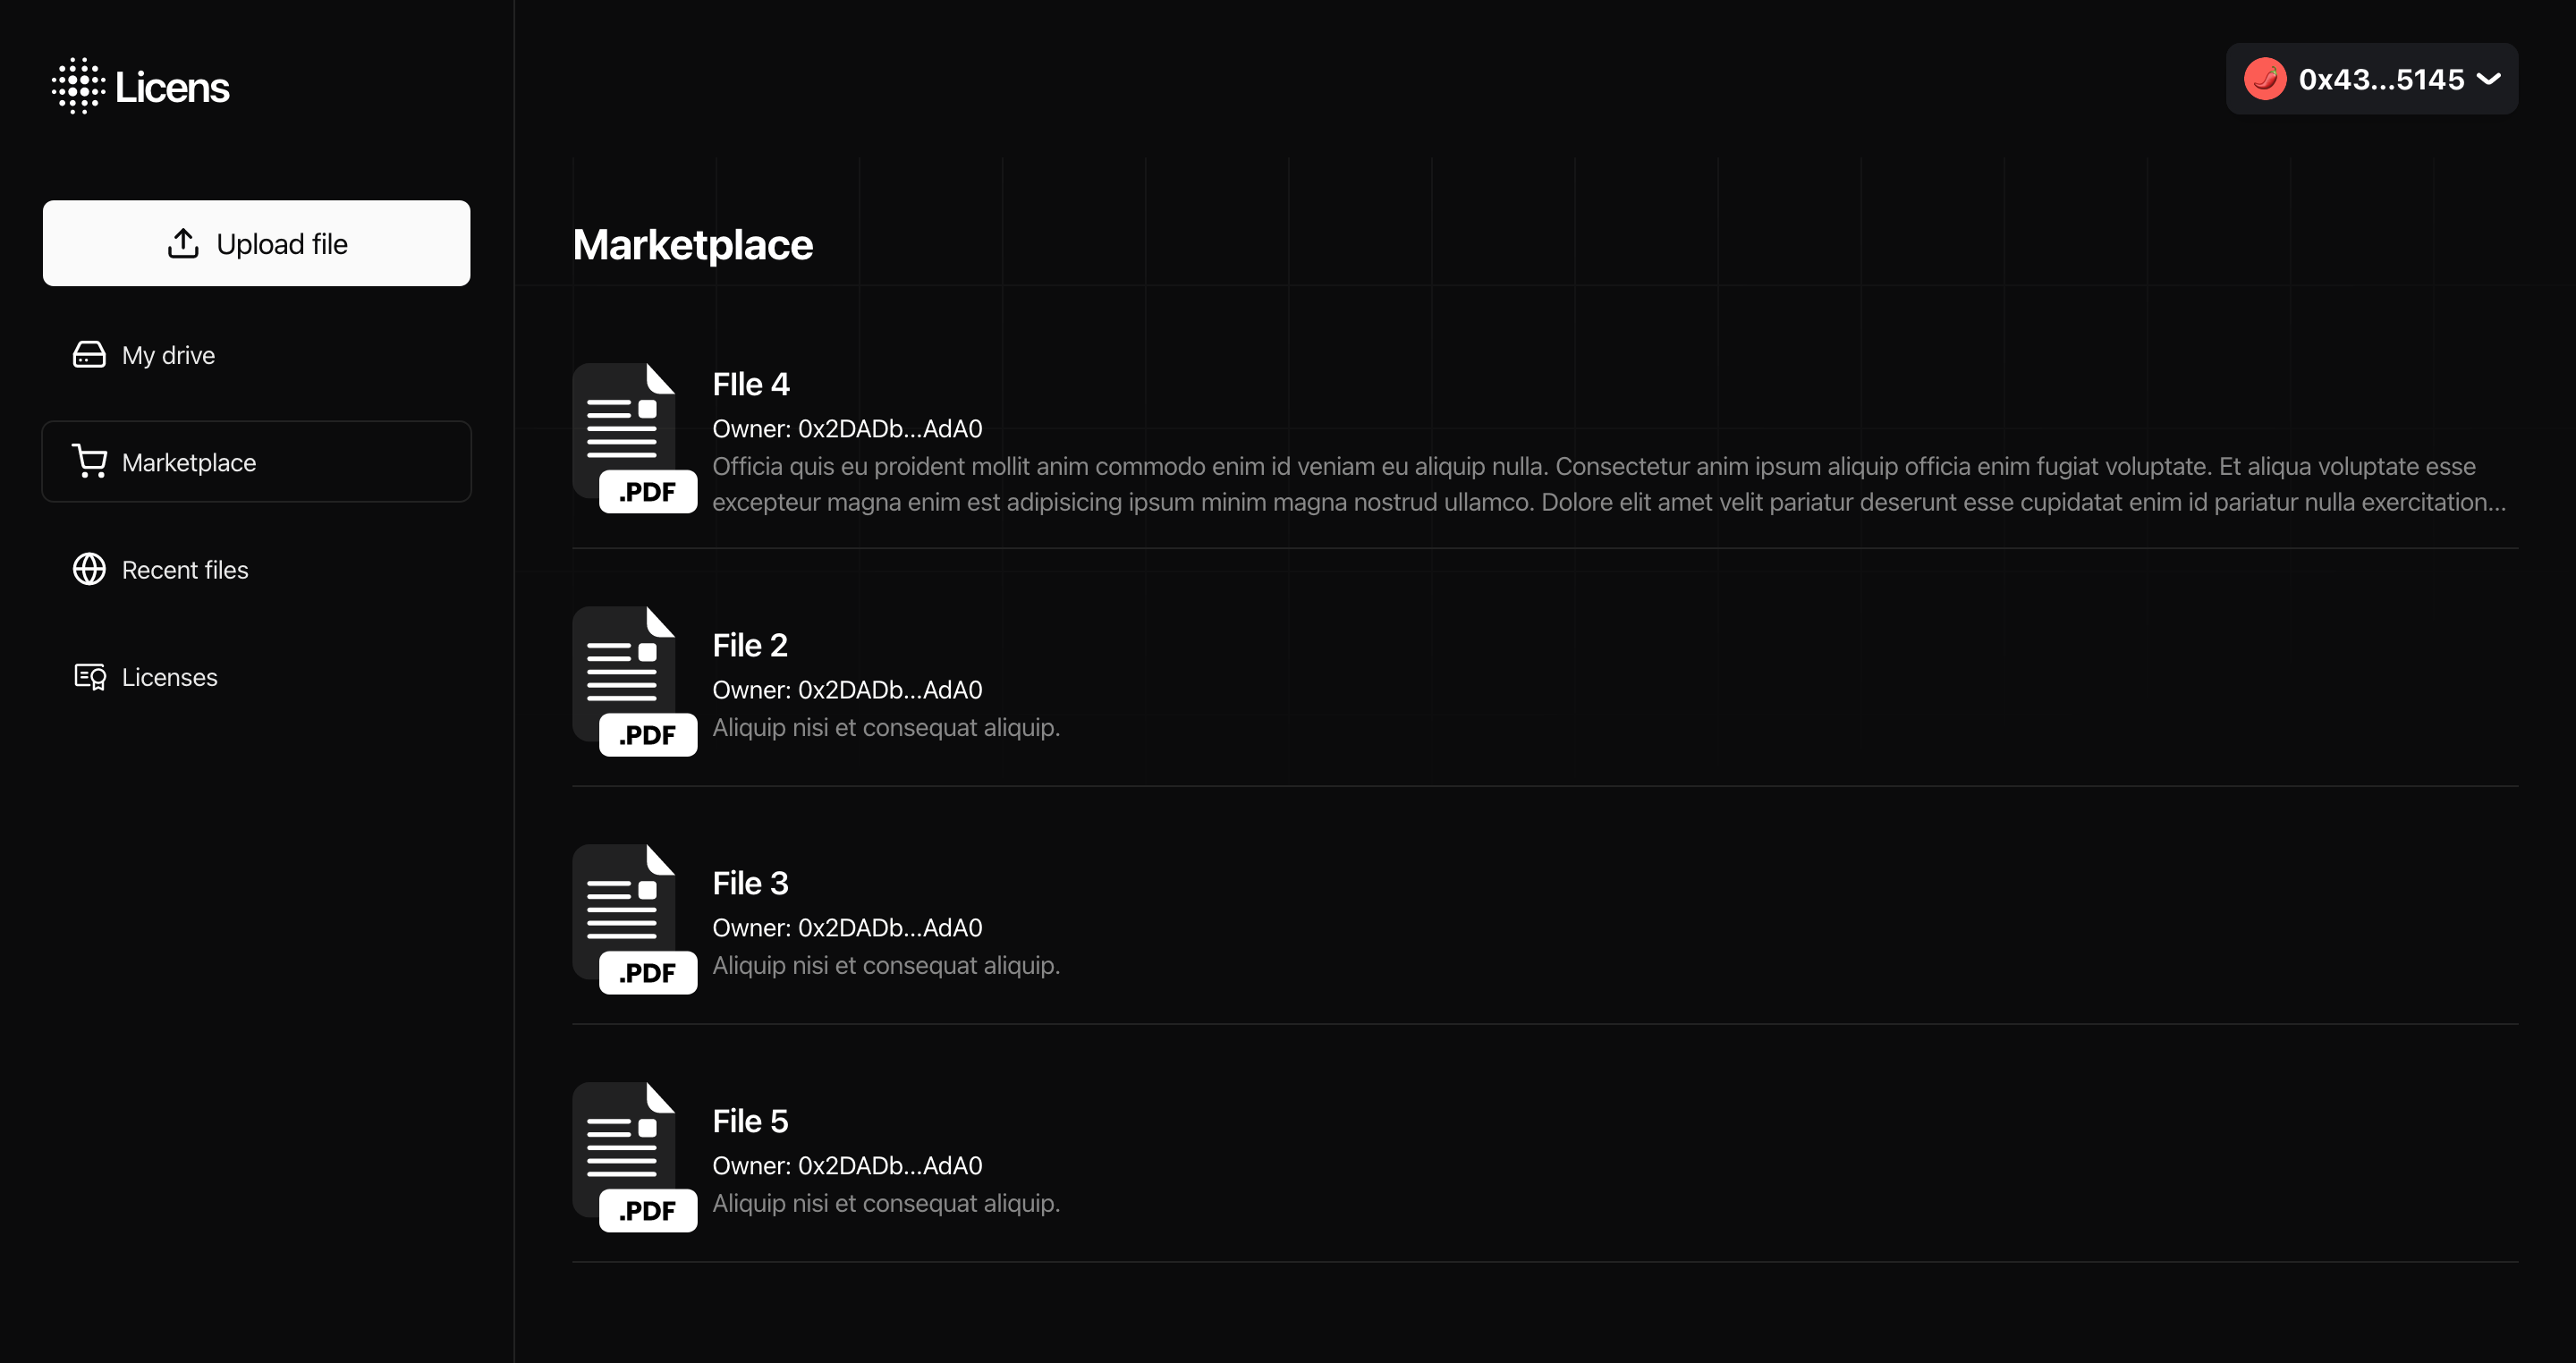
\includegraphics[scale=0.165]{src/images/marketplace-page.png}
	\caption{}
\end{figure}

\begin{figure}[h!]
	\centering
	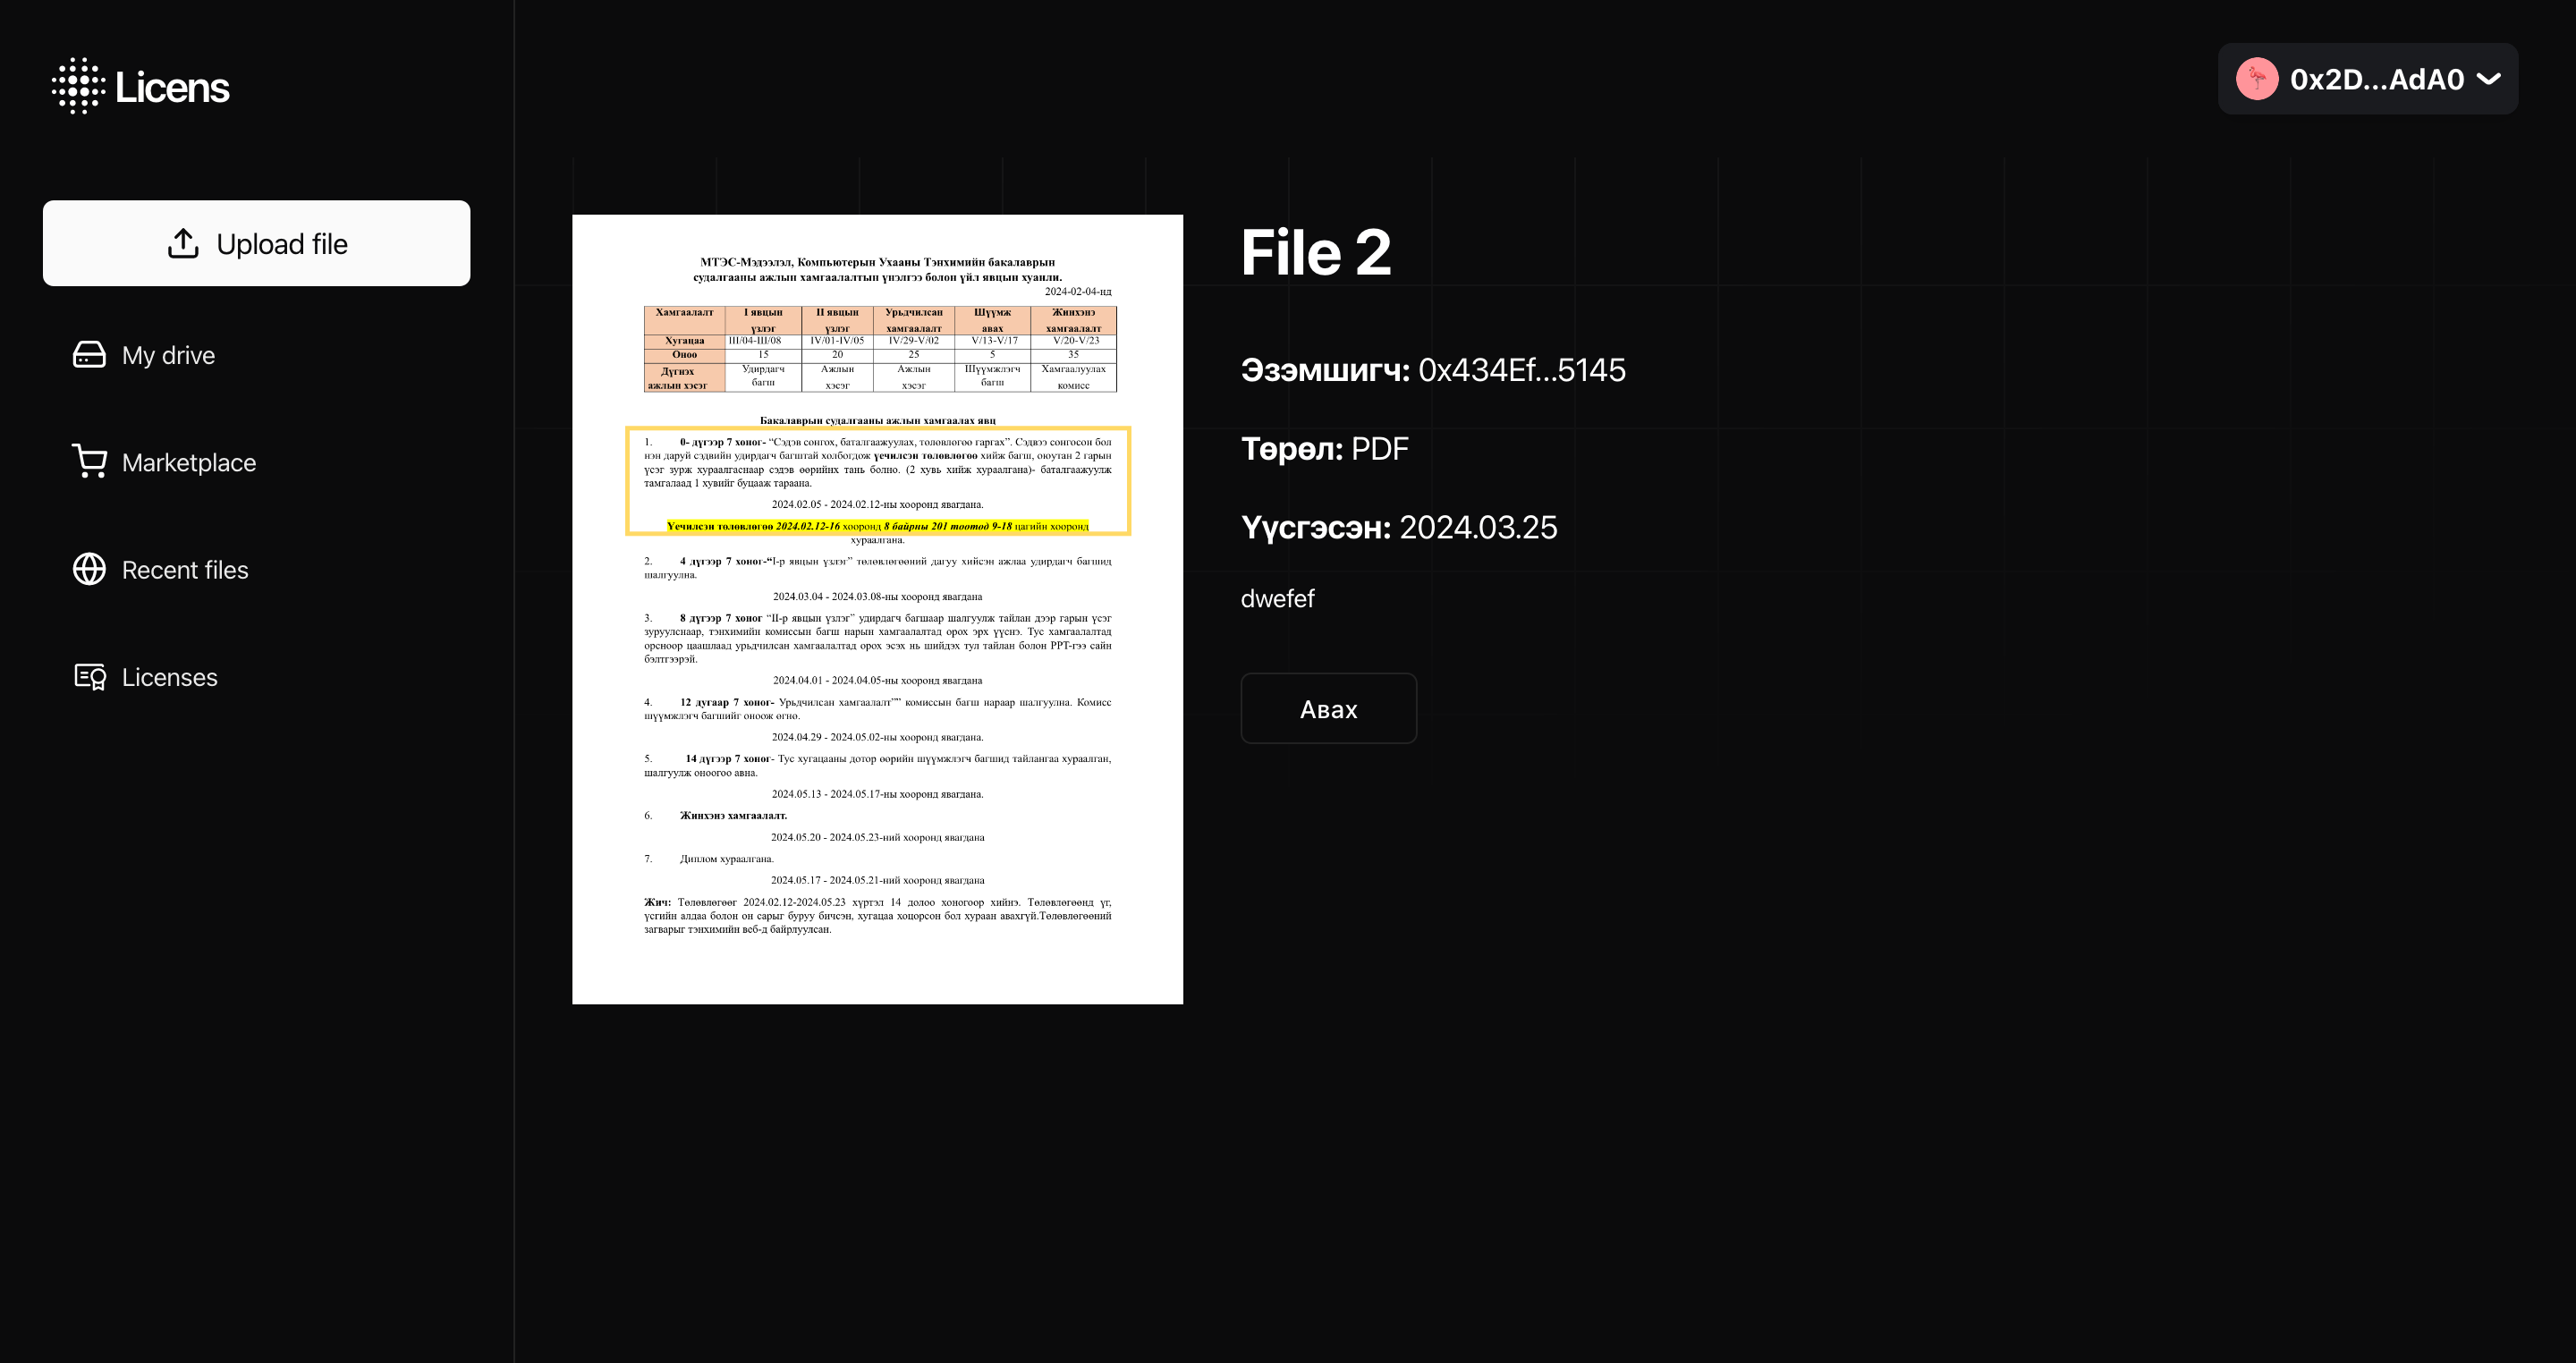
\includegraphics[scale=0.165]{src/images/file-page.png}
	\caption{}
\end{figure}

%----------------------------------------------------------------------------------------
%   Дүгнэлт эндээс эхэлнэ
%----------------------------------------------------------------------------------------
\chapter{Дүгнэлт}
Энэхүү судалгааны ажлаар блокчэйн технологи болон дижитал эрхийн менежментийн талаар судласан. Энэхүү судалж суралцсан мэдлэгээ ашиглан практикт цахим бүтээлийн лицензийн систем бүтээхийг зорилоо. Хөгжүүлэлтийн явцад блокчэйн сүлжээнд цахим бүтээлийг байршуулах, лиценз олгох, лицензийн баталгаажуулалт зэрэг янз бүрийн функцүүдыг хэрэгжүүлж, туршиж үзсэн.
\\
Үр дүнд нь орчин үеийн шинэлэг блокчэйн технологиудтай танилцсан ба бүтээгдэхүүний шаардлагыг гаргаж ухаалаг гэрээ бичихээс эхлээд эцсийн хэрэглэгчид хүрэх чанарын шаардлагыг хангаж блокчэйн технологийг ашиглан найдвартай, ил тод, төвлөрсөн бус системийг бүтээлээ.


%----------------------------------------------------------------------------------------
%   Дипломын номзүй, хавсралтын хэсэг эндээс эхэлнэ
%----------------------------------------------------------------------------------------

\singlespace
\addcontentsline{toc}{part}{НОМ ЗҮЙ}
\begin{thebibliography}{}
	% Ашигласан материалыг эндээс оруулна
   \bibitem{blockchain}
   Adam Hayes, Blockchain Facts: What Is It, How It Works, and How It Can Be Used. (December 15, 2023) \url{https://www.investopedia.com/terms/b/blockchain.asp}
   \bibitem{dlt}
   Scott Nevil, Distributed Ledger Technology (DLT): Definition and How It Works. (May 31, 2023) \url{https://www.investopedia.com/terms/d/distributed-ledger-technology-dlt.asp}
   \bibitem{zug_digtal_id}
    Sundararajan S. UN Agencies Turn to Blockchain In Fight Against Child Trafficking. (Nov 13, 2017)  \url{https://www.coindesk.com/markets/2017/11/13/un-agencies-turn-to-blockchain-in-fight-against-child-trafficking/}
   \bibitem{zug_digtal_id}
   Zug Digital ID: Blockchain Case Study for Government Issued Identity.  \url{https://www.investopedia.com/terms/b/blockchain.asp}
   \bibitem{drm}
   What is digital rights management (DRM)?.  \url{https://business.adobe.com/blog/basics/digital-rights-management}

\end{thebibliography}
\appendix
\addcontentsline{toc}{part}{ХАВСРАЛТ}

% Хавсралтын нэр. Хавсралт гэдэг үг агуулахгүй
\chapter{Үечилсэн төлөвлөгөө}
\begin{figure}[h!]
   \centering
   \includegraphics[scale=0.065, angle=90]{src/images/periodic-plan.png}
   \caption{Удирдагчийн үнэлгээ дүгнэлт}
\end{figure}


\chapter{Кодын хэрэгжүүлэлт}
\lstinputlisting[language=TypeScript, caption=Ухаалаг гэрээ,basicstyle=\linespread{0.6}\ttfamily,frame=single]{src/code/smart-contract.sol}

Уг код нь хэрэглэгчийн оруулах цахим бүтээлийг  мэдээллийг блокчэйнд бичнэ.
\lstinputlisting[language=TypeScript, caption=Блокчэйнд бичих,basicstyle=\linespread{0.8}\ttfamily,frame=single]{src/code/writeFile.ts}


Уг код нь хэрэглэгчийн оруулсан цахим бүтээлийн мэдээллийг блокчэйнээс уншина.
\lstinputlisting[language=TypeScript, caption=Блокчэйнээс унших,basicstyle=\linespread{0.8}\ttfamily,frame=single]{src/code/getUserFiles.ts}



%----------------------------------------------------------------------------------------
%   Хавсралтууд эндээс эхэлнэ
%----------------------------------------------------------------------------------------

\end{document}
